\documentclass[12pt,a4paper]{article}
\usepackage[utf8]{}
\usepackage[T1]{fontenc}
\usepackage[utf8]{inputenc}
\usepackage{amsmath}
\usepackage{amssymb}
\usepackage[hidelinks]{hyperref}
\usepackage{graphicx}
\usepackage{caption}
\usepackage[shortlabels]{enumitem}
\usepackage{listings}
\usepackage{courier}
% \usepackage{fontspec}
% \newfontfamily\UbuntuMonospace{Ubuntu Mono}
% \listfiles
\usepackage{pythonhighlight}
\hypersetup{colorlinks = true}
\date{Sommersemester 2022}

\renewcommand{\baselinestretch}{1.1}
\renewcommand{\familydefault}{\rmdefault}
\renewcommand{\thesection}{} 
\renewcommand{\arraystretch}{1.3}
\setlength\parindent{0pt}

\setlength{\hoffset}{-18pt}         
\setlength{\oddsidemargin}{0pt} % Marge gauche sur pages impaires
\setlength{\evensidemargin}{0pt} % Marge gauche sur pages paires
\setlength{\marginparwidth}{54pt} % Largeur de note dans la marge
\setlength{\textwidth}{481pt} % Largeur de la zone de texte (17cm)
\setlength{\voffset}{-18pt} % Bon pour DOS
\setlength{\marginparsep}{7pt} % Séparation de la marge
\setlength{\topmargin}{0pt} % Pas de marge en haut
\setlength{\headheight}{13pt} % Haut de page
\setlength{\headsep}{4pt} % Entre le haut de page et le texte
\setlength{\footskip}{27pt} % Bas de page + séparation
\setlength{\textheight}{720pt} % Hauteur de la zone de texte (25cm)

\lstdefinestyle{mystyle}{
    basicstyle=\ttfamily\footnotesize,
    breakatwhitespace=false,         
    breaklines=true,                 
    captionpos=b,                    
    keepspaces=true,                
    showspaces=false,                
    showstringspaces=false,
    showtabs=false,                  
    tabsize=2
}
\bibliographystyle{abbrv}
\lstset{style = mystyle}
\usepackage{natbib}
\usepackage{graphicx}

\begin{document}
%__________________________________________Titel dieser Sitzung___________________________________________________

\title{Masterarbeit - Protokoll}
\author{Vincent Kather}
\maketitle
\vspace{5 cm}
\hypersetup{linkcolor=black}
\tableofcontents
\listoffigures
\listoftables
\hypersetup{linkcolor=red}
\newpage

\newpage
\section{Papers}
\addtocounter{section}{1}
Datum: 4.Mai \ 

\noindent\hrulefill  \

%__________________________________________Inhalt dieser Sitzung__________________________________________________

\subsection{Humpback whale song hierarchical structure: Historical context and discussion of current classification issues } % (fold) 
\label{sub:Cholewiak-2013-Marine Mammal Science}

\begin{itemize} 
  \item humpback whale songs hypothesized to play a role in female attraction or mediate male-male interactions \cite{cholewiak_humpback_2013}
  \item four core features have been observed:
  \begin{enumerate}
    \item populations of males that are in acoustics contact sing similar songs
    \item hierarchical structure is observed globally, details vary following isolation of populations from one another
    \item song patterns change over time resulting from indivieual males modifying the spectral and temporal features of units, as well as order and repetition
    \item males in acoustics contact include similar changes in songs, even as these change over time
  \end{enumerate}
  \item variations in song units and patterns, are important for understanding the function of song within this species and the influence of sexual selection on singing behavior
  \item "There is clearly a need for the development of automated classification systems in order to handle large data sets of recordings; however, no system has yet been demonstrated which compares with the pattern recognition skills of the human brain." - ich bin dran
    \begin{itemize}
      \item song session          $\Longrightarrow$  series of songs with pauses less than a minute
      \item song                $\Longrightarrow$  combination of multiple distinc themes
      \item theme             $\Longrightarrow$  similar phrases comprise a theme
      \item phrase          $\Longrightarrow$  set of units
      \item subphrase     $\Longrightarrow$  sequence of one or more units, sometimes repeated in series
      \item motif       $\Longrightarrow$  units of repetition 
      \newline \indent $\hookrightarrow$ similar:     containing only one type of unit
      \newline \indent $\hookrightarrow$ dissimilar:  containing two or more different units, repeated in combination
      \item unit      $\Longrightarrow$  shortest continuous sound
      \item subunit $\Longrightarrow$  pulses to rapid to be individually discriminated
    \end{itemize}

  \item syllables is ambiguous and thus shouldn't be used, instead use unit
  \item die unterteilung in phrases ist sehr subjektiv, da zusammengehörigkeiten nicht objektiv begründet werden können
  \item desplite challenges in labeling and delineating phrases, phrase duration is very stable over years compared to songs and other structural elements
  \newline \indent $\hookrightarrow$ strongly suggests, that phrases are essential elements of communication to humpback whales

  \item guideline to delineating phrases:
  \begin{enumerate} 
    \item consectutive units, similar structure shouldn't be seperated within a phrase but bundled as parts of a subphrase
    \item phrases should be seperated so that there is not an incomplete phrase at the end of a sequence
    \item transitional phrases entail units of two different phrase types, which subphrases occur previously and subsequently. 
      \newline \indent $\longrightarrow$ Example: ab ab ab ad cd cd cd
      \newline \indent $\longrightarrow$ in this case the ad woule be the transitional phrase
    \item care should be taken when trying to distinguish between a inherent variation within a phrase and changing of units, structure or composition to a point where the definition of a new phrase seems more sensible
      \newline \indent $\longrightarrow$ spectrograms should be provided to support the decision
    \item phrase duration should be measured from the onset of one phrase until the onset of the subsequent phrase
      \newline \indent $\longrightarrow$ variation within phrase duration is the smallest compared to that of other structures within a population
    \item phrase delineation should always be based on recordings of multiple individuals rather than a single isolated individual 
  \end{enumerate}

  \item fundamental theme is a concept that is ephemeral as so much changes between seasons
  \item Payne and Payne:
  \begin{itemize} 
    \item static themes:       sequence of nearly identical phrases
    \item shifting themes:     successive phrases evolve from one to the other
    \item unpatterned themes:  variable number of units lack organisation cannot be subdivided into repeating phrases  ---> rather rare
      \newline \indent $\longrightarrow$ theme consists of a single non repeated phrase
  \end{itemize}
  \item structure can be preserved over the span of several years, even though the individual units undergo changes
  \item song structure is sometimes cyclical, meaning that one theme always leads to another and in the end back to the first, this is however only sometimes the case
  \item there seems to be a general rule of certain themes leading to other themes, however, exceptions to the rule do exist
  \item in bird singing literature, songs are identified as having longer pauses between them compared to elements within the song
  \item song birds might be a working analogon to humpback themes
  \item song length increased due to acoustic disturbances 
  \newline \indent $\hookrightarrow$ although there are opposing results
  \newline \indent $\longrightarrow$ seeing that the song duration metric is complicated, singers could also increase the number of repetitions due to the occurrence of noise
  \newline \indent $\longrightarrow$ increases in song duration are more likely the result of more variation in theme sequences, singing themes that would not otherwise occur sequentially before arriving back at the beginning, if there is a beginning
  \newline \indent $\longrightarrow$ as soon as theme order is less stable, quantifying a song length becomes difficult
  \newline \indent $\hookrightarrow$ the underlying problem is, that the definition of a song is vague, is it the occurrence of a specific theme labeled as 'beginning', is it a sequence of individual themes? this decision greatly impacts song duration and theme composition within a song
  \newline \indent $\hookrightarrow$  if the theme order is invariant song definition is more stable and the subsequent metrics of song duration make sense, if however theme order is variant and no hierarchy seems apparent the meaning of a 'song' and the consequential metrics are problematic
  \item males seem to switch between different phrase types a lot more in the presence of another singer
  \newline \indent $\longrightarrow$ similar observations on birds might indicate an escalation of aggression between two males
\end{itemize}

\newpage
\subsection{Garland-2020-Frontiers in Psychology} % (fold)
\label{sub:garland_2020_frontiers_in_psychology}
\begin{itemize}
  \item study of bird songs has provided information on learning mechanisms \cite{garland_cultural_2020}
  \newline \indent $\longrightarrow$ songs are learned rather than inherited
  \item understanding of cultural evolution through social learning and underlying hormonal and neural pathways
  \item production learning: a form of social learning, resulting from experience with signals of other individuals, an animal learns to modify the form of its own signal
  \newline \indent $\longrightarrow$ considered rare in vertebrates (wirbeltiere)
  \item only one songbird species has a way of creating new songs on a yearly bases, similar to humpbacks $\Longrightarrow$ the corn bunting (Emberiza (Miliaria) calandra)
  \item whether songs serve the purpose of finding a mate, male-male interaction, or multi-message signal is still debated
  \item humpback songs sessions can last for many hours
  \item it's assumed that there is a worldwide inherited repertoire of song units, and new songs are still comprised of these units but changed in their order and structure
  \item humpbacks are considered to be \textit{eventual variety} singers $\Longrightarrow$ the repeat phrases before moving to the next theme
  \item males in a given population will sing the same song type
  \newline \indent $\hookrightarrow$ strong cultural conformity
  \item no song has reappeared (since recording started)
  \item the changing and creating of new songs and what individual plays a key role is still elusive
  \item song sharing occurs for three reasons:
  \begin{enumerate}
     \item sharing through shared breeding grounds/migratory routes
     \item sharing through males visiting more than one wintering ground in consecutive years
     \item sharing through males visiting more than one breeding ground within a breeding season
   \end{enumerate} 
   \item \textit{song revolution} $\Longrightarrow$ song from one population appears in other population and rapidly replaces it entirely
  \newline \indent $\longrightarrow$ this process occurs regularly with songs taking 2 years to spread from east Australia, where they emerge all the way to French Polynesia
  \item in South Pacific several songs can be existent at the same time
  \item in North Pacific populations are more constrained by landmasses, thus fewer variations in songs coexist
  \item new songs appear to spread from larger populations to smaller ones
  \item the quest for novelty is driven by sexual selection, however it is constrained, otherwise empirical findings would show much more diversification of songs
  \item a \textit{switch when similar} rule seems to guide the application of new songs
  \newline \indent $\hookrightarrow$ changes from old to new songs happen at units that are similar in both old and new
  \newline \indent $\hookrightarrow$ at the same time a remembering of last seasons song seems to exist, preventing the humpback from switching to old songs even though units are similar
  \newline \indent $\longrightarrow$ similar discrimination processes exist in songbirds learning process
  \item while a song evolves, it increases in complexity, only to be replaced by a far simpler song in the next \textit{song revolution}
  \item song complexity may resemble cognitive skills and thus used by prospective mates
  \item differences between corn buntings and humpbacks song learnings:
  \begin{itemize}
    \item corn bunting songs change evolutionary $\Longrightarrow$ new songs have similarities with old songs
    \newline \indent $\hookrightarrow$ humpback song changes are revolutionary $\Longrightarrow$ new songs have not similarities with old songs
    \item population size of birds is roughly 100 s and for humpbacks is 1000-40000
    \newline \indent $\hookrightarrow$ humpback songs transported tens of kms
    \newline \indent $\longrightarrow$ bird songs reach tens of males, humpback songs reach hundreds of males
    \newline \indent $\hookrightarrow$ for high fidelity audio humpbacks would need to be within 10 km of source to pick up on high freq information, so audience size might be comparable 
    \item new songs can come from isolated males from other populations for humpbacks, whereas they come from within the same population for corn buntings
    \item corn buntings song change seems to be triggered by reproductive success i.e. successful males will most likely be copied from by other birds
    \newline \indent $\longrightarrow$ mating success is not as obvious for humpbacks and thus a less likely metric to decide whom to copy
    \newline \indent $\hookrightarrow$ research for humpback still in progress, one hypothesis states that whales might try to interrupt singers that escort a female and if they fail to succeed in interrupting them, they instead copy from them 
  \end{itemize}
  \item similarities between corn buntings and humpbacks:
  \begin{itemize}
    \item similar song structures
    \item song evolution (of the same song) is most probably the result of production errors in both species
    \newline \indent $\hookrightarrow$ however does not explain revolutions
  \end{itemize}
  \item whether humpback songs convey fitness information that females use in mate choice is an open research question
  \item decreasing population sizes for corn buntings may also influence the origin of new songs
  \newline \indent $\hookrightarrow$ flourishing population sizes for many humpback populations might influence song learning in a different way 
  \item "Unfortunately, no songbird or any other animal species to date have exhibited the rapid and repeated population-wide replacement of a cultural phenotype as observed in humpback song revolutions."
  \item a comparison between humpback song revolutions and rapid cultural change in human pop music and slang change might be worth looking into
\end{itemize}
    
% subsection garland_2020_frontiers_in_psychology (end)
\newpage
\subsection{Terrestrial, Semi-aquatic, and Fully Aquatic Mammal Sound Production Mechanisms} % (fold)
\label{sub:terrestrial_semiaquatic_and_fully_aquatic_mammal_sound_production_mechanisms}
\begin{itemize}
  \item Author: Joy S. Reidnberg \cite{reidenberg_terrestrial_2017}
  \item odontocedes can use echolocation sounds for navigation and prey tracking
  \item all mammals use pneumatic machanisms to generate sounds
  \item larynx evolved to keep water out of a buoyancy organ in fish
  \newline \indent $\longrightarrow$ today its main function remains protective, but in terrestrial mammals it prevents incursions of foreign material into the lungs
  \item vocal cords, as well as cartilages act as splashguards, deflecting food and water away from the opening. They interlock the larynx with the rear of the nasal vacity
  \newline \indent $\longrightarrow$ this interlock channels airflow through the larynx and seperates it from the swallowing pathway $\Longrightarrow$ this division of airspace allows breathing and swallowing $\Longrightarrow$ a crucial feat to detect predetors while feeding
  \item one of the last features to be added to the larynx was phonation $\Longrightarrow$ producing the fundamental frequency of vocalizations
  \item the vocal cords are rather folds, stacked tissue of varying density periodically compressing air
  \newline \indent $\longrightarrow$ the geometry of the supralaryngeal vocal tract (vocal tract downstream of larynx) adds resonances and thus harmonics of the fundamental frequency
  \newline \indent $\hookrightarrow$ vocal folds are the source, supralaryngeal vocal tract is the filter
  \item semiaquatic mammals (spend time both on land and in water: hippopotamus, seal, polar bear, otters, etc.) keep their vocal folds shut under water to prevent drowning
  \newline \indent $\longrightarrow$ most solely vocalize on land
  \newline \indent $\hookrightarrow$ exception: hippopotamus and pinnipeds (seals, sea lions, walruses)
  \begin{itemize}
     \item hippos produce sounds in air and underwater
     \item hippos have their vocal folds oriented parallel (rather than perpendicular) to the tracheal airflow
     \item this anatomy is similar to their close relatives the cetaceans
     \item hippos can produce sounds with their moths open without being in danger of drowning
     \newline \indent $\longrightarrow$ their orientation of vocal folds alongside tall vartilages tha interlock the larynx with the nasal cavity protects agains water intake
     \item pinnipeds vocal folds may be oriented parallel (seal lion) or perpendicular (seal) to the tracheal airflow
     \newline \indent $\hookrightarrow$ open-mouthed vocalizations are dangerous $\Longrightarrow$ vocaliation mostly occurs when the mouth is closed 
   \end{itemize} 
   \item fully aquatic mammals (sirenians (manatees and gugongs) and cetaceans) produce sound nearly exclusively underwater
   \begin{itemize}
     \item U shaped pair of vocal folds oriented parallel to tracheal airflow 
     \item if the front of the larynx is closed, air is led through epiglottic and corniculate cartilages $\Longrightarrow$ diversion of airflow
     \newline \indent $\longrightarrow$ airflow causes fold vibrations, leading to low-frequency sounds
     \newline \indent $\longrightarrow$ air can be recycled for next vocalizations
     \item if the front of the larynx is opened, vocal folds are closed, air passes above the epiglottis and between piared flaps of corniculate cartilage
     \newline \indent $\longrightarrow$ flaps may clap together and produce pulsed sounds
     \item the respiratory tract of cetaceans has evolved unlike that of sirenians, causing cetaceans to be able to vocalize with open mouths, whereas sirenians can't
     \item unlike terestrial mammals, cetaceans primarily utilize surrounding tissues rather than air in the supralaryngeal vocal tract to carry vibrations through neck and head outwards
     \newline \indent $\longrightarrow$ the density of the surrounding tissues is similar to that of seawater, thus smaller loss in transmission due to change in impedance
     \item mysticetes and odontocetes have developed differing sound generation mechanisms, as they have evolved along different trajectories.
     \newline \indent $\longrightarrow$ mysticetes produce infrasound
     \newline \indent $\longrightarrow$ odontocetes produce ultrasound
     \item mysticetes and odontocetes have undergone an evolutionary divergence as their vocal folds are both parallel to the tracheal airflow but 180° reversed
     \item \textbf{Mysticetes:}
     \begin{itemize}
       \item primarilly produce infrasound to be able to communicate over vast distances
       \item similar to other mammals mysticetes produce sound laryngeally
       \item have evolved tall corniculate cartilages that also protext the larynx from behind, creating a circumferential protection around the larynx
       \newline \indent $\longrightarrow$ food and water are swallowed past the larynx but cannot slip through and end up accidentally inhaled
       \item larynx is larger than either one of the whales lungs
       \newline \indent $\longrightarrow$ larynx volume and surface area allows for loud and low-frequency sounds, amplified by larger resonant volumes corresponding with longer wavelengths and increased amplification
       \item Laryngeal sac also plays a crucial role in respiratory and buoyancy control
       \item laryngeal sac is expanded as air is used to vocalize and contracted, sending the air back to the lungs to be reused for vocalization
       \item diving whales decending to deep depths require large volumes as the increase in ambient pressure with decending decreases the air volume, resulting in limited abilities in terms of amplification and low-frequency sound generation
       \item Laryngeal sac walls can vibrate, transferring the vibrations through the overlying throat muscles, blubber, and skin into the surrounding water
       \item opposite the laryngeal opening, a pair of tissue flaps can be clapped together to generate pulsed sounds
       \newline \indent $\longrightarrow$ clapping, a more broadband, especially high frequency containing signal, can be used to echolocate
       \item video of mysticete larynx: \url{https://youtu.be/rysR5SNwrn8}
       \item see fig. \ref{fig:sound_prod_mysticetes}
     \end{itemize}
     \item \textbf{Odontocetes:}
     \begin{itemize}
       \item generate high frequency sounds used for navigation and finding prey
       \item use the nasal region to generate clicks
       \item too have a complex structured larynx with an undetermined function
       \newline \indent $\longrightarrow$ echolocation sounds are produced in the nasal region
       \newline \indent $\hookrightarrow$ larynx might be important for production of communication sounds, not however for echolocation
       \item odontocete larynx can be open while protecting the respiratory tract. shape is similar to snorkel.
       \newline \indent $\longrightarrow$ the complexity of the larynx suggests that it must have an essential and nearly constant role for airflow, and as no breathing is occurring underwater its most likely necessary for $\Longrightarrow$ sound production.
       \newline \indent $\hookrightarrow$ the level of protection is superior to that of mysticetes, allowing odontocetes to swim upside down while making noises and still not getting water into the respiratory tract
       \item Sound production through the larynx is theoretically possible (yet never observed or recorded!) through three options:
       \begin{enumerate}
         \item air flows through the larynx and causes vibrations of laryngeal tissue
         \item air is simply channeled constantly to the nasal region to be used for sound generation there
         \item elevating the larynx to increase pressure in the nasal cavity, driving air upward through sound-generating tissues located there. (previously observed through endoscopy)
       \end{enumerate}
       \item the nostrils of odontocetes have fused to become a single blowhole, unlike mysticetes who have a pair of blowholes
       \item below the nostril are two nasal passageways and a complex arrangement of air sacs, nasal plugs and fatty structures. 
       \newline \indent $\longrightarrow$ the epicranial (above skull) structures (homologous to facial tissue) comprise muscles controlling nasal plugs, to prevent water from entering, the other structures aid sound generation
       \newline \indent $\hookrightarrow$ they are made up of: bilaterally paired sets of air sacs, fatty structure (melon), and two sets of paired fat bodies (phonic lips $\Longrightarrow$ sonar sources)
       \item phonic lips can clap against each other when air passes between them, or it can produce whistles when air passes along their ridges
       \item Sperm whales only have one of these pair of lips \url{https://www.youtube.com/watch?v=sW7o5IC2io0}
       \item Dolphins, having two pairs of lips can produce different clicks simultaneously or whistle and click simultaneously
       \item downstream of the phonic lips, air is guided through three pairs of air sacs, located underneath the blowhole
       \newline \indent $\longrightarrow$ the blowhole is closed during this process
       \item air sacs are inflated allowing for longer airflow for sound production (same in mysticetes)
       \newline \indent $\longrightarrow$ like in mysticetes, air is reused several times for sound production
       \item high vibration speeds of phonic lips generate ultrasonic clicks, that are transmitted as vibrations to attached fat bodies (dorsal bursae)
       \newline \indent $\longrightarrow$ vibrations are carried through the anterior dorsal bursa to a contiguous larger fat body in the forhead (melon)
       \item the melon is a biconvex shaped organ, made up of isovaleric acid (saturated fatty acid), with similar density as seawater (small loss due to impedance change)
       \newline \indent $\longrightarrow$ the isovaleric acid or spermaceti is one of the reasons it was heavily hunted as the huge amounts of the fatty acid was used in cosmetics, lubricant, and expecially candles
       \item the shape of the melon can be altered through facial muscles, thus focusing the direction of the sound beam  
       \item see fig. \ref{fig:sound_prod_odonto}
     \end{itemize}
     \item "The divergence into opposite ends of the frequency spectrum highlights how these two taxa, although related, pursued very different niches for their acoustic abilities."
   \end{itemize}
\end{itemize}

\begin{figure}
  \centering
  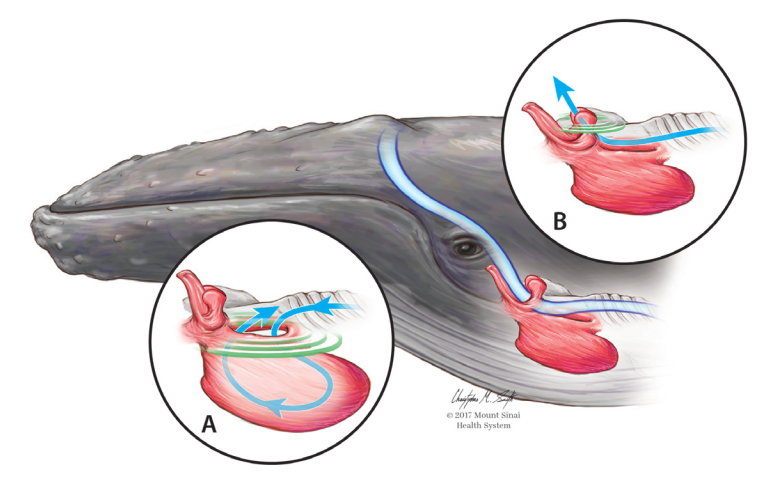
\includegraphics[width=.5\linewidth]{Images/sound_prod_mysticetes.png}
  \caption[Sound production in Mysticetes.]{Sound production in Mysticetes. A: Larynx is closed, air is lead into laryngeal sac, airflow diversion causes low frequency vibrations. B: epliglottic cartilage is closed, corniculate cartilage open, causing air to pass through it. Corniculate cartilage can be closed periodically causing pulsed sounds.}
  \label{fig:sound_prod_mysticetes}
\end{figure}

\begin{figure}
  \centering
  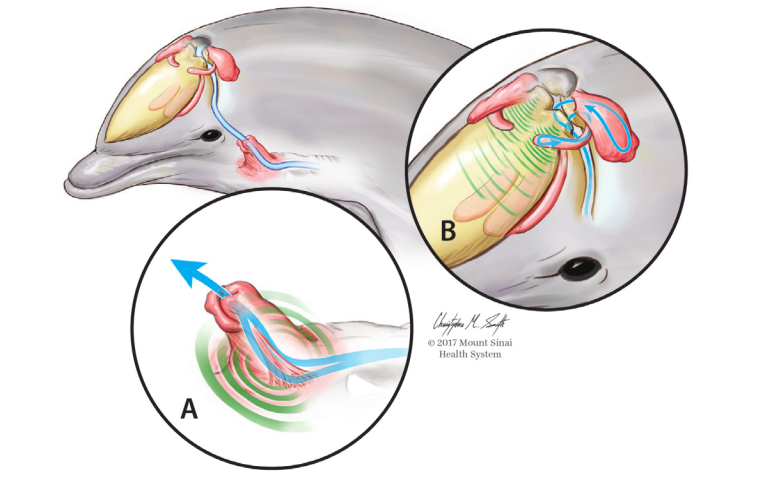
\includegraphics[width=.5\linewidth]{Images/sound_prod_odontocetes.png} 
  \caption[Sound production in Odontocetes]{Sound production in Odontocetes. A: larynx evolved in a way to ideally protect respiratory tract from water and can potentially aid in sound production (though never observed). B: highly compex nasal ragion able to produce loud ultrasonic clicks and whistles used for ecolocation.}
  \label{fig:sound_prod_odonto}
\end{figure}
% subsection terrestrial_semiaquatic_and_fully_aquatic_mammal_sound_production_mechanisms (end)

\newpage
\subsection{The devil is in the detail: Quantifying vocal variation in a complex, mulit-levelled, and rapidly avolving display} % (fold)
\label{sub:the_devil_is_in_the_detail_quantifying_vocal_variation_in_a_complex_mulit_levelled_and_rapidly_avolving_display}

\begin{itemize}
  \item Author: Ellen C. Garland and Luke Rendell \cite{garland_devil_2017}
  \item \textit{song types} - different versions of a song, alterations in themes and phrases
  \item the unidirectionality in song transmission is not well understood, however it is possible to use diffrences in the song to identify different dialects and also poulations at any point in time.
  \item aiming to quantify similarities between different humpback whale songs, the Levenshtein distance (LD) has outperformed all other metrics, \ref{ssub:levenshtein_distance}
  \newline \indent $\longrightarrow$ the LD is a robust metric, preferable to Markov chains, Markov hidden models, or Shannon entropy
  \item to ensure comparable outcomes between different lengthened strings, the LD is standardised by the length of the longer string in the pair, LD similarity index:
  \begin{equation}
    \text{LSI}(a, b) = 1- \frac{\text{LD}(a, b)}{\text{max}(\text{len}(a), \text{len}(b))}
  \end{equation}
  \item as the LD only compares but doesn't account for the different levels of hierarchy in the humpback song, an additional weighting system is proposed
  \item all recorded units were compared which reduced the 750 recorded units to 96 unique units
  \newline \indent $\hookrightarrow$ units were subjected to Classification and Regression Tree analysis, \textbf{CARF} as well as Random Forest trees
   \item CART 77\% and RF 73\% classification overlap with human classifiers
   \item to cluster data, the average of each variabel (ex. maximum frequency) was calculated and z-transformed
   \item 11 acoustic features were extracted and Euclidian distance was calculated based on them
   \newline \indent $\longrightarrow$ features: Duration, $f_{min}$, $f_{max}$, $f_{start}$, $f_{end}$, $f_{range} = f_{max}/f_{min}$, $f_{trend} = f_{start} / f_{end}$, Bandwidth $f_{max} - f_{min}$, Inflections (Wendpunkte) $\text{count}(\ddot f(t) =0)$, $f(\text{mag}_{max})$, Pulse rate
   \item the normalized Euclidian distance was calculated:
   \begin{equation}
     d(x, y) = \frac{\sqrt{\Sigma_i (z(x_i) - z(y_i))^2}}{\mathrm{max}(d)}
   \end{equation}
   \item d was used as a weighting penalty for substitutions in LD calculations
   \newline \indent $\longrightarrow$ with linear d, very different units were off the scale and similar units very unpenalized, making comparisons unpractical
   \newline \indent $\hookrightarrow$ introduction of exponential normalized cost: exp\_cost$(x, y) = 1- e^{- \beta d(x, y)}$, with $\beta = [1, 0.5, 0.25]$
   \item $\beta = 1$ is close to unweighted (everything = 1),  $\beta = 0.25$ comes closet to linear weighing
   \item other options of weighting systems would be penalty matrix based on the output of node weights, Euclidian distances, or Cartesian distances
   \item as phrase duration has proven to be one of thee most stable components of humpback whale song, insertions and deletions are more heavily penalized than subsitutions
   \item analysis was practiced on 3 levels:
   \begin{enumerate}[A]
     \item a string represents a sequence of units, assigning them to a phrase
     \item a string represents a sequence of units to identify a median unit sequence per phrase/theme, this is the sequence with the highest summed similarity (LSI) to all other members within the group
     \newline \indent $\longrightarrow$ this provides a representative string for the set that can be used to compare among sets
     \item a string represents a sequence of phrases (song) assigning them to a song type
   \end{enumerate}
  \indent $\longrightarrow$ C is only based on unweighted analyses
    \item to attain sampling distributions, the data is bootstrapped with multi-scale bootstrap resampling 1000 times
    \newline \indent $\longrightarrow$ AU significance: p > 95\%
    \newline \indent $\longrightarrow$ BP significance: p > 70\%
    \item when first analyzed with unweighted LD, similarity between 4 chosen representative themes was single digit percentages, similarity within a theme (comparing median phrase with other phrases) was between 44 \% and 73 \%, and increased to 53 \% to 79 \% once $\beta=1$ weighting was applied.
    \item because phrase length was chosen as important and substitutions are less penalized by lower $\beta$ weighting values, a threshold exists, where phrase length is considered more important than actual similarity, as substitutions are less penalized than deletions and insertions.
    \newline \indent $\longrightarrow$ insertions and deletions maintained penalty scores of 1, and substitution penalty scores needed to exceed 0.6 to manage this phenomenon
    \item the study shows that weighting schemes offer a methodology to prefer one kind of similarity over others, however, all weighting schemes come with consequences and researchers should be cautious of the way research questions are framed and if the weighting scheme really favors it
    \item many different methods can be used to favor certain substitutions over others, i.e. every euclidian distance over 0.5 leads to a substitution penalty of 1 
    \item ultimately weighting of LD analyses will aid in clarifying fine-scale differences between humpback songs, potentially helping to find dialects and theme progressions.
    \item the usage of median strings can be used to find the most representative phrase for each theme (intra-individual) and these can then be compared to other individuals to understand differences in cultural diversity within a population
    \newline \indent $\longrightarrow$ ANOVA (\ref{ssub:analysis_of_variance_anova}) could be used to further explore diversity
\end{itemize}

% subsection the_devil_is_in_the_detail_quantifying_vocal_variation_in_a_complex_mulit_levelled_and_rapidly_avolving_display (end)
\newpage
\subsection{Deep Machine Learning Techniques for the Detection and Classification of Sperm Whale Bioacoustics} % (fold)
\label{sub:deep_machine_learning_techniques_for_the_detection_and_classification_of_sperm_whale_bioacoustics}
\begin{itemize}
  \item authors: Peter Bermant, Michael Bronstein \cite{bermant_deep_2019}
  \item cateceans pose an important taxa to study langauge, as the difference in environment  can be revealing from a comparative perspective in regards to aquatic communication
  \item sperm whales mainly communicate through codas - 3-40 broadband clicks that are in general transmitted in socializing groups
  \item aside from communicative codas, sperm a variety of click-baed sounds exist:
  \begin{enumerate}
    \item usual clicks for echolocation and foraging
    \item foraging for short-range prey detection and feeding
    \item reverberating slow clicks (clangs) produced only by mature males
  \end{enumerate}
  \item NN applied in 4 ways:
  \begin{enumerate}
    \item detection of echolocation clicks using CNN
    \item classification of codas into categorical types using a Long Short-Term Memory (LSTM) RNN-based approach
    \item recognition of coval clan coda dialects with LSTM RNNs
    \item identification of individual whales based on coda production with LSTM RNNs
  \end{enumerate}
  \item LSTM RNNs are effective for this because their architectures aebanle the network to preserve the non-independent sequential order of input data
  \item 99.5\% train accuracy with 650 spectrogram images (325 click and no-click)
  \newline \indent $\longrightarrow$ echolocation classification task works very well with the CNN approach
  \item For LSTM RNN classification of different cods, a network is pretrained on a proxy-task (a task similar to the final task, but requiering less data), this is called \textbf{self-supervised learning}
  \newline \indent $\longrightarrow$ in this case learning the time interval between subsequent clicks
  \item utiziling transfer learning procedures, the network is then trained on coda type, vocal clan and individual whale identity classification
  \item first perform PCA for dimensionality reduction from 256 to 20, then t-SNE to reduce from 20 to 3
  \item results from both echolocation and coda classification were very postive
\end{itemize}
% subsubsection deep_machine_learning_techniques_for_the_detection_and_classification_of_sperm_whale_bioacoustics (end)

\newpage
\subsection{Acoustic Detection of Humpback Whales Using a Convolutional Neural Network} % (fold)
\label{sub:acoustic_detection_of_humpback_whales_using_a_convolutional_neural_network}
\begin{itemize}
  \item Ann N. Allen \cite{allen_convolutional_2021}
  \item second author Matt Harvey, Software Engineer, Google AI Perception 
  \item some have tried power law approaches, to review power in frequency bands and detect based on that, the abundance of other noises in the ocean however, makes this approach less practical
  \item 187000h of recordings, with the technique of active learning, to increase the training set size
  \item recordings orifinate from 13 sites in the North Pacific, using bottom-mounted High Frequency Acoustic Recording Pachages (HARPs), equipped with omni-directional hydrophones, with a flat ($\pm 2$dB) hydrophone sensitivity from 10 Hz to 100 kHz (with -200dB V/$\mu$Pa)
  \item monitoring duration varied from a month, to 13 years
  \item recording schedules ranging from continuous to 5 min of every 40 min
  \item recording files consisted of 75 s blocks of audio (\textit{segments})
  \item deployment depths $\in [111, 1266]m$, avg = 730m
  \item raw data sampled at 200 kHz, low-pass filtered at 10Hz, resampled at 10 kHz
  \newline \indent $\longrightarrow$ effective bandwidth: [10, 5000] Hz (13 TB of data)
  \item binary classification task, based on a image classification CNN model
  \item model results were compared to energy-based detectors as a baseline
  \item per channel energy normalization (PCEN) was applied to the spectrograms 
  \item spectrogram creation:
  \begin{itemize}
    \item STFT with Hann window of length 1024 samples (100 ms)
    \item output size: 128 x 96 (txf)
    \item strides of 10, 30, 50 ms
    \item along f axis, trials binned using a triangular mel filterbank over squared FFT magnitudes
    \item three different amplitude compression functions were used: log, root compression and PCEN
    \newline \indent $\longrightarrow$ PCEN: normalizing by componentwise dividing the STFT with temporally smoothed version of the same STFT and then apply root compression
    \newline \indent $\hookrightarrow$ smoothing is done for each channel independently, smoothing constant: s = 0.04
  \end{itemize}
  \item the model was based on the architecture by Hershey et al. (2017) found best at detecting audio event classes in YouTube videos
  \newline \indent $\longrightarrow$ ResNet-50 CNN with a lowered stride from 2 to 1 of the initial 7x7 conv layer (images are smaller than on the original model)
  \item data augmentation happened on-the-fly, with time shift by $\pm$16 bins relative to non-overlapping grid, done dynamically so perturbations were varied accross epochs
  \item \textbf{active learning}
  \begin{itemize}
    \item iterative strategy that improves an existing classifier by using it to selec the most valuable examples for additional human annotation and subsequent retraining
    \item model predictions were reevaluated to speed up anotation process and at the same time throw out negatives that were close calls (boat noise, minke whale calls)
    \newline \indent $\longrightarrow$ resulting audited data: 291.8 h of reviewed recordings for train, test, and validation set
  \end{itemize}
  \item baseline performances were set by a reimplemented generalized power-law detection algorithm for humpbacks (GPL) and a simple band-limited energy detector
  \item results: average precision = 0.97, AUC-ROC = 0.992
\end{itemize}
% subsubsection acoustic_detection_of_humpback_whales_using_a_convolutional_neural_network (end)

\newpage
\subsection{All units are equal in humpback whale songs, but some are more equal than others} % (fold)
\label{sub:all_units_are_equal_in_humpback_whale_songs_but_some_are_more_equal_than_others}
\begin{itemize}
  \item by Eduardo Mercado III \cite{mercado_all_2022}
  \item controvertial author
  \item quotes from George Orwells animal farm in title
  \item claims that contrary to most other researchers, units are not constant throughout the years
  \item because units are not constant, and they vary in the distance over which they are audible, the theory of the humpback whales song being solely for sexual selection and display of intellectual capacity does not hold
  \item Mercado argues that the frequencies in units are precisely chosen and altered to generate sonar that can give information about changing environments and prey
  \item 
\end{itemize}
% subsection all_units_are_equal_in_humpback_whale_songs_but_some_are_more_equal_than_others (end)

%____________________________________________Ende dieser Sitzung__________________________________________________

\newpage
\section{Examples}
\addtocounter{section}{1}
Datum: 12.05.22 \ 

\noindent\hrulefill  \

%__________________________________________Inhalt dieser Sitzung__________________________________________________

\subsection{Statistics} % (fold)
\label{sub:Statistics}

\subsubsection{Bootstrapping Dendrograms} % (fold)
\label{ssub:bootstrapping_dendrograms}
Paper: Bootstrap confidence levels for phylogenetic trees
\url{https://www.pnas.org/doi/10.1073/pnas.93.23.13429?url_ver=Z39.88-2003&rfr_id=ori:rid:crossref.org&rfr_dat=cr_pub%20%200pubmed}
\begin{itemize}
  \item procedure:
  \begin{enumerate}
    \item collect data and arrange it in \textbf{x} so that
    \begin{itemize}
      \item rows correspond to different species
      \item columns correspond to sequence
      \newline \indent $\longrightarrow$ humpback units, phrases, letters of a word ...
    \end{itemize}
    \item create distance matrix \textbf{D}
    \begin{itemize}
      \item distance matrix has dimensions (len(x) x len(x))
      \item quantify distance of each row with each other row using a distance metric like LD \ref{ssub:levenshtein_distance}
    \end{itemize}
    \item create phylogenetic tree
    \begin{itemize}
      \item use connection algorithm to cluster elements, one clustering per generation, reducing the size of the distance matrix by one/generation
    \end{itemize}
  \end{enumerate}
  \item this procedure is then repeated with bootstrapped datasets:
  \begin{itemize}
    \item a bootstrapped datamatrix \textbf{x*} is created using the same rows but the columns are randomly selected from \textbf{x}
  \end{itemize}
  \item this way trees are built in the same manner several hundred times
  \item the proportions of bootstrap trees resulting in the same topology with the original are calculated
  \newline \indent $\longrightarrow$ these proportions are bootstrap confidence values or \textbf{bootstrap probability (BP)}
  \newline \indent $\hookrightarrow$ so the numbers on merging branches indicate the percentage in how many cases these were merged together at that stage 
  \item the underlying assumption of course is that columns, so sequence elements are independent of another, questionable if this holds for humpback whale units
  \item the underlying idea behind bootstrapping is to use the observed data \textbf{x} and the bootstrappend data \textbf{x*}, attain estimates $\mathbf{\hat \theta^*}$ and $\mathbf{\hat \theta}$ and calculate $\mathbf{\hat \theta^*} - \mathbf{\hat \theta}$ to then get a probability and a standard deviation, telling us that knowing $\mathbf{\hat \theta^*} - \mathbf{\hat \theta}$ we can estimate $\mathbf{\hat \theta} - \mathbf{\theta}$ with the same margin of error (= std from $\mathbf{\hat \theta^*} - \mathbf{\hat \theta}$)
  \newline \indent $\longrightarrow$ $\hat \theta$ in this case is the observed phenomenon and $\theta$ is the phenomenon
\end{itemize}
% subsubsection bootstrapping_dendrograms (end)


\subsubsection{ANOVA} % (fold)
\label{ssub:anova}
\begin{itemize}
  \item from wikipedia: goal: find out what factors play into the weight of a dog aat a dog show
  \item a dog show has numerous dogs on display
  \item a histogram of all dog weights is made
  \item first approach would be to divide the dogs based on characteristics hoping, that the decomposition into its aspects will yield correlations
  \item each group should have a low variance of dog weights and the mean of the groups should be distinct, so that the make up for different parts of the overall histogram
  \newline \indent $\longrightarrow$ analogous to a fourier transformation - dissecting a group into its fundamental components
  \item in a first attempt the group was split by age and length of hair, then by pet and working breed, and finally by breed
  \newline \indent $\longrightarrow$ the first two options both yield 4 resulting groups ($2^2$) whereas the last one yields as many groups as there are breeds
  \item the last option is the most feasable in this case, because the last one had the most distinct means and no overlap, see fig. \ref{fig:anova}
  \newline \indent $\longrightarrow$ the group histograms of the last split are \textbf{linear independent}
\end{itemize}

\begin{figure}
  \centering
  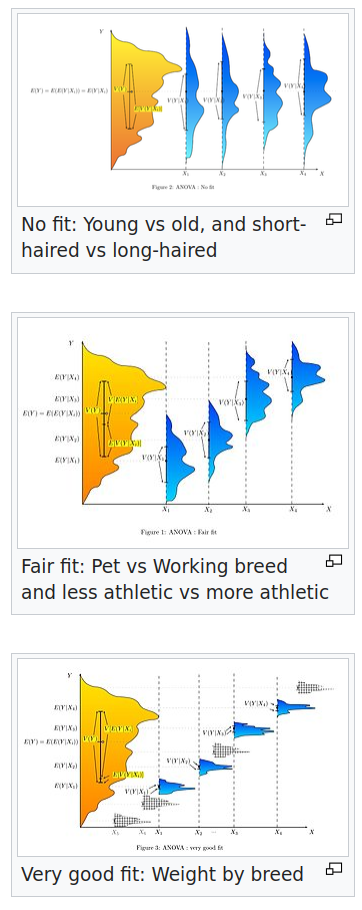
\includegraphics[width=.3\linewidth]{Images/ANOVA.png}
  \caption[ANOVA example: dog weights]{ANOVA example: dog weights. Different attempts to find the factors underlying dog weights. The last example is the best fit, because all histograms distinct and don't overlap.}
  \label{fig:anova}
\end{figure}
% subsubsection anova (end)

\subsection{Machine Learning} % (fold)
\label{sub:machine_learning}

\subsubsection{Perceptron training} % (fold)
\label{ssub:perceptron_training}

training a perceptron with scikit learn:
\begin{python}
  import numpy as np
  from sklearn.datasets import load_iris
  from sklearn.linear_model import Perceptron
  iris = load_iris()
  X = iris.data[:, (2, 3)] # petal length, petal width
  y = (iris.target == 0).astype(np.int) # Iris Setosa?
  per_clf = Perceptron()
  per_clf.fit(X, y)
  y_pred = per_clf.predict([[2, 0.5]])
\end{python}
% subsubsection perceptron_training (end)

% subsection machine_learning (end)

%____________________________________________Ende dieser Sitzung__________________________________________________


\newpage
\section{Statistics}
\addtocounter{section}{1}
Datum: 11.05.22 \ 

\noindent\hrulefill  \

%__________________________________________Inhalt dieser Sitzung__________________________________________________

\subsection{Transformations} % (fold)
\label{sub:Transformations}

\subsubsection{Z-Transformation (also standardization or auto-scaling)} % (fold)
\label{ssub:z_transformation_also_standardization_or_auto_scaling_}

% subsubsection z_transformation_also_standardization_or_auto_scaling_ (end)
\begin{itemize}
  \item a \textbf{z-score} (standard score) calculates the distance of a given point from the mean in multiples of the std
  \item z-Scores become comparable by measuring in multiples of std of sample
  \newline \indent $\longrightarrow$ \textbf{mean of z-transformed data is always 0}
  \newline \indent $\longrightarrow$ \textbf{std of z-transformed data is always 1} (if original distribution is normal)
  \item ex. see fig. \ref{fig:z-trafo}
\end{itemize}

\begin{figure}
  \centering
  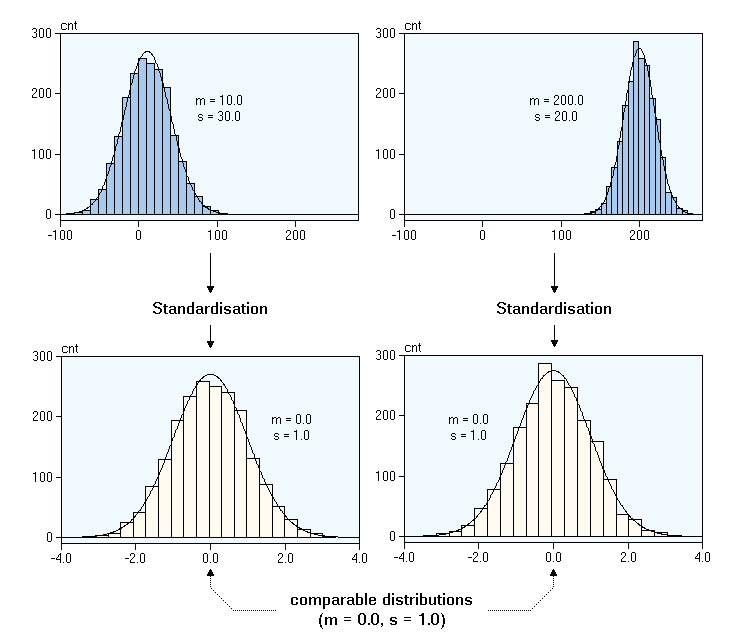
\includegraphics[width=.5\linewidth]{Images/z-trafo.png}
  \caption[Example of z-transformation]{Example of z-transformation. unique distribution of data point relative to one another is preserved, but mean and std are standardized.}
  \label{fig:z-trafo}
\end{figure}

\subsubsection{Unweighted Pair Grouped Method with Arithmetic Mean - UPGMA} % (fold)
\label{ssub:unweighted_pair_groupd_method_with_arithmetic_mean_upgma}
\begin{itemize}
  \item the clusters with the smallest distance between them are clustered and the distance matrix is recalculated
  \newline \indent $\longrightarrow$ the distance between two clusters is the average pair wise distance of all objects within both clusters
  \begin{equation}
    d_{(A \cup B), X} = \frac{|A| d_{A,X} + |B| d_{B,X}}{|A| + |B|}
  \end{equation}
  \indent $\longrightarrow$ where $d_{(A \cup B), X}$ is the distance between the new cluster $A \cup B$ and X, and $|A|$ denotes the size of A
\end{itemize}
% subsubsection unweighted_pair_groupd_method_with_arithmetic_mean_upgma (end)

\subsubsection{Bootstrapping} % (fold)
\label{ssub:bootstrapping}
\begin{itemize}
  \item bootstrapping is a statistical method that resamples a single data set to create many simulated samples
  \item bootstrapped samples have the same size as the original but will have some data points more than once and others not at all
  \newline \indent $\longrightarrow$ bootstrapping assumes that the existing data set is a accurate representation of the actual population
  \item using computers datasets are bootstrapped thousands of times, when plotting the resulting distribution of mean values of the sampled data a normal distribution will occur, (almost) regardless of the distribution in the data set
  \newline \indent $\longrightarrow$ this is called a sampling distribution of means (if calculated analytically its a probability distribution)
  \newline \indent $\hookrightarrow$ if the top and bottom 2.5 \% are cut off, we are left with a 95 \% confidence interval, meaning that the mean of our original sample dataset will lie within that interval with a probability of 95 \% 
\end{itemize}
% subsubsection bootstrapping (end)


\subsubsection{Phylogenetic tree} % (fold)
\label{ssub:phylogenetic_tree}
\begin{itemize}
  \item phylogenetic trees, or evolutionary trees are branching diagrams showing the evolutionary relationships among various biological species based on similarities and differences in physical or genetic characteristics
  \item Dendrograms
  \begin{itemize}
    \item dendrograms are representations of trees used in \textbf{hierarchical clustering}, computational biology, and phylogenetics
    \newline \indent $\longrightarrow$ hierarchical clustering can be \textbf{Agglomerative} - bottom-up; or \textbf{Divisive} - top-down
    \newline \indent $\hookrightarrow$ bootstrapping is a Agglomerative approach 
  \end{itemize}
  \item \textbf{bootstrapping dendrograms}
  \begin{itemize}
    \item data points are merged, one per generation, reducing the data matrix by one dimension per generation
    \newline \indent $\longrightarrow$ mergers are evaluated using tests:
    \begin{itemize}
      \item bootstrap probability (BP) value: computed by normal bootstrap resampling, see \ref{ssub:bootstrapping_dendrograms} (much simpler than AU)
      \newline \indent $\longrightarrow$ BP is the frequency that a value appears in the bootstrap replicates
      \item approximately unbiased (AU) p-value: computed by multi scale bootstrap resampling proving a superior approximation to unbiased p-values
      \newline \indent $\longrightarrow$ text
    \end{itemize}
    \item when picturing the clustering process, there exists a boundary that has to be overcome for the merger to happen. So the clustering process is a distance measurement in a 2 dimensional space
    \item while BP is equivalent to assuming a flat Bayesian prior for $\mu$ (an clustering candidate is equally possible to lie anywhere within the space), AU takes into account the shape of the boundary between both states and is thus a more precise measure
    \item while the boundary between the two states can be a straight line, it can also be a circle due to radial conditions (for the straight line case BP and AU are identical, for the circular boundaries they are not)
    \item AU requires higher bootstrapping rates than BP
    \item BP is said to have a downward bias, though this is disputed
  \end{itemize}
  \item CCC is a metric to quantify the overall associations within the data by the dendrogram see \ref{ssub:cophenetic_correlation_coefficient}
\end{itemize}
% subsubsection phylogenetic_tree (end)





\subsection{Metrics} % (fold)
\label{sub:metrics}

\subsubsection{Levenshtein Distance} % (fold)
\label{ssub:levenshtein_distance}
  \begin{itemize}
    \item LD is a string metric 
    \newline \indent $\longrightarrow$ measures distance between two text strings for approximate string matching or comparison (used in fuzzy string searching), must satisfy the triangle inequality (two sides of a triangle must be greater or equal to third side)
    \item LD between two words is the minimum number of single-character edits required to change one word into the other
    \item definition:
    \begin{equation}
      \text{lev}(a, b) = \begin{cases}
        |a| & \text{ if } |b| = 0 \\
        |b| & \text{ if } |b| = 0 \\
        \text{lev} (\text{tail}(a), \text{tail}(b)) & \text{ if } |a| = |b| \\
        1 + \begin{cases}
          \text{lev} (\text{tail}(a), b) \\
          \text{lev} (a, \text{tail}(b)) \\
          \text{lev} (\text{tail}(a), \text{tail}(b))
          
        \end{cases} & \text{ otherwise }
      \end{cases}
    \end{equation}
      \newline \indent $\longrightarrow$ tail is a string lacking the first element, |*| denote length of string
  \end{itemize}
% subsubsection levenshtein_distance (end)

\subsubsection{Cophenetic Correlation Coefficient} % (fold)
\label{ssub:cophenetic_correlation_coefficient}
\begin{itemize}
  \item CCC is a measure how faithfully a dendrogram (tree diagram often used in taxonomy) preserves the pairwise distances between the unmodeled data points
  \newline \indent $\longrightarrow$ CCC > 0.8 is considered high and thus a good representation of associations within the data
\end{itemize}
% subsubsection cophenetic_correlation_coefficient (end)


% subsection metrics (end)

\subsection{Tools} % (fold)
\label{sub:tools}

\subsubsection{statistical significance} % (fold)
\label{ssub:statistical_significance}
\begin{itemize}
  \item a result has statistical significance when it is very unlikely to have occurred given the null hypothesis ($H_0$)
  \item the significance level, $\alpha$, is the probability of a study to reject $H_0$ if given $H_0 == $ True
  \newline \indent $\longrightarrow$ $\alpha$ is a measure of the strength of the evidence that must be present in your sample before you will reject $H_0$ and call the effect statistically significant
  \newline \indent $\longrightarrow$ $\alpha$ is determined before the experiment
  \begin{itemize}
    \item p-value in null-hypothesis significance testing is the probability of obtaining test results at least as extreme as the result observed, given that $H_0 ==$ True
    \item small p-value $\Longrightarrow$ extreme observed outcome would be very unlikely under $H_0$
    \newline \indent $\longrightarrow$ lower p-values indicate greater evidence against $H_0$
    \newline \indent $\longrightarrow$ p-values help in determining which hypothesis the data supports
  \end{itemize}
  \item if $p \le \alpha$ you can reject $H_0$ and conclude the event is statistically significant $\Longrightarrow$ the evidence in your sample is strong enough to be able to reject $H_0$ at population level
  \newline \indent $\longrightarrow$ conventionally $\alpha = 5\%$ or lower, depending on the field of study
\end{itemize}
% subsubsection statistical_significanc (end)


\subsubsection{z-test} % (fold)
\label{ssub:z_test}
\begin{itemize}
  \item a z-test determines whether two population means are different when the variances are known an the sample size is large (>30)
  \newline \indent $\longrightarrow$ normal distribution and knowledge of std are required
  \begin{equation}
    Z = \frac{\bar X - \mu_0}{\sigma}
  \end{equation}
  \newline \indent $\longrightarrow$ $\bar X$ is mean of sampled data, $\mu_0$ is the expected value, $\sigma$ is the std
  \item after the z-score is calculated it gets evaluated in the hypothesis test, where it's compared to the value chosen in the null- and alternative hypotheses 
  \item 
\end{itemize}
% subsubsection z_test (end)

\subsubsection{Two-Tailed Test} % (fold)
\label{ssub:two_tailed_test}
\begin{itemize}
  \item used in null-hypothesis testing and testing for statistical significance
  \item used when a hypothesis states that a sample is either significantly greater or less than the mean of a population
  \item depending on how critical consequences are, conventions can either require the number of data points that must exist within the acceptance range to be 5\% (1.96) or 0.001\%
  \newline \indent $\longrightarrow$ the acceptance range is also referred to as alpha
\end{itemize}
% subsubsection two_tailed_test (end)

\subsubsection{Analysis of Variance - ANOVA} % (fold)
\label{ssub:analysis_of_variance_anova}
\begin{itemize}
  \item ANOVA is an analysis tool that splits an observed accumulated variability found inside a data set into two parts
  \begin{itemize}
    \item systematic factors: have a statistical influence on the data set
    \item random factors: don't have an influence on the data set
  \end{itemize}
  \item ANOVA can be used to determine the influence that independent variables have on the dependent variables in a regression study
  \item ANOVA is the extension of the t- and z-tests
  \begin{equation}
    F = \frac{\text{MST}}{\text{MSE}}
  \end{equation}
  \newline \indent $\longrightarrow$ F = ANOVA coefficient, MST = Mean sum of squares due to changes, MSE = Mean sum of squares due to error
  \item ANOVA is used to test the difference between two or more means
\end{itemize}
% subsubsection analysis_of_variance_anova (end)

% subsection tools (end)

%____________________________________________Ende dieser Sitzung__________________________________________________




\newpage
\section{Machine Learning}
\addtocounter{section}{1}
Datum: 11.05.22 \ 

\noindent\hrulefill  \

%__________________________________________Inhalt dieser Sitzung__________________________________________________

\subsection{Algorithms} % (fold)
\label{sub:Algorithms}

\subsubsection{Decision Tree} % (fold)
\label{ssub:decision_tree}

% subsubsection decision_tree (end)
\begin{itemize}
  \item hierarchical structure with binary division based on single feature and threshold
\end{itemize}

\subsubsection{Random Forest} % (fold)
\label{ssub:random_forest}

% subsubsection random_forest (end)
\begin{itemize}
  \item train a group of Decision Tree classifiers, each on a different random subset of the training set
  \item Predictions are made by getting all predictions of the individual trees and predicting the class with the most votes
  \newline \indent $\longrightarrow$ even though its simple it's one of Machine Learnings most powerful algorithms
  \newline \indent $\longrightarrow$  Ensemble Learning algorithms like random forests are good to use near the end of a project, once you have already built a few good predictors to combine them into a very good predictor
  \newline \indent $\hookrightarrow$ winning ML solutions often involve several Ensemble methods
\end{itemize}

\subsubsection{Classification and Regression Tree - CART} % (fold)
\label{ssub:classification_and_regression_tree_cart}

% subsubsection classification_and_regression_tree_cart (end)
\begin{itemize}
   \item set is split into two parts based on one feature and one corresponding threshold
   \newline \indent $\longrightarrow$ feature and threshold are chosen to produce the purest subsets (weighted by their size)
   \item the algorithm then minimizes the following cost function:
   \begin{equation}
     J(k, t_k) = \frac{m_{left}}{m}G_{left} + \frac{m_{right}}{m}G_{right}
   \end{equation}
   \newline \indent $\longrightarrow$ with $G_{left/right}$ - measure of impurity of the left/right subset
   \newline \indent $\longrightarrow$ and $m_{left/right}$ - number of instances in left/right subset
   \item algorithm works recursively, splitting into smaller and smaller sets until no minimization is reached or maximum depth is achieved
   \newline \indent $\hookrightarrow$ CART is a \textit{greedy algorithm} - greedily searches for optimum split at each level, regardless of consequential impurity at lower levels; \textit{greey algorithms} produce reasonably good results, not optimal ones. Finding optimal trees is a NP-Complete Problem $\Longrightarrow$ requires $O(\exp(m))$ time, so reasonably good must be settled for
 \end{itemize} 

\subsubsection{Principal Component Analysis - PCA} % (fold)
\label{ssub:principal_component_analysis_pca}

% subsubsection principal_component_analysis_pca (end)
\begin{itemize}
  \item PCA is the most popular dimensionality reduction algorithm
  \item PCA requires a centered dataset around the origin (Scikit-Learn does this automatically, others dont)
  \item a principal component is the $i_{th}$ unit vector yielding the largest amount of variance (they are orthogonal)
  \item PCA uses the principal components to create a plane closest to the data points
\end{itemize}

\subsubsection{t-Distributed Stochastic Neighbor Embedding (t-SNE)} % (fold)
\label{ssub:t_distributed_stochastic_neighbor_embedding_}
\begin{itemize}
  \item unsupervised, non-linear technique primarily used for data exploration and visualizing high-dimensional data
  \item contrary to PCA, t-SNE preserves only small-pariwise distances or local similarizies whereas PCA only preserves large pairwise distances
  \item Swiss Role example, works well with t-SNE not so much with PCA
  \item t-SNE algorithm calculates a similarity measure between paris of instances in high and low dimensional space and tries to optimize both similarity measures using a cost fucntion.
  \begin{enumerate}
    \item measure similarities between points in high dimensional space
    \newline \indent $\longrightarrow$ perform gaussian distribution around all the points, calculate density for every point, renormalize $\Longrightarrow$ get probabilities for each point, which are proportional to the similarity meaning points with similar values, they will be similar
    \item repeat 1. but use Student t-distribution with only 1 degree of freedom (Cauchy distribution) instead of gaussian distribution, see fig. \ref{fig:cauchyguas}. This gives us a set of probabilities in the low dimensional space
    \item we want the two sets of probabilities to be similar, so: measure the difference between the distributions using \textbf{Kullback-Liebler divergence} (asymmetrical approach, for efficient comparisons) and use gradient descent to minimize the KL cost function.
  \end{enumerate}
  \item an important distinction from PCA is that t-SNE alters the inputs, so its only for exploration
\end{itemize}
\begin{figure}
  \centering
  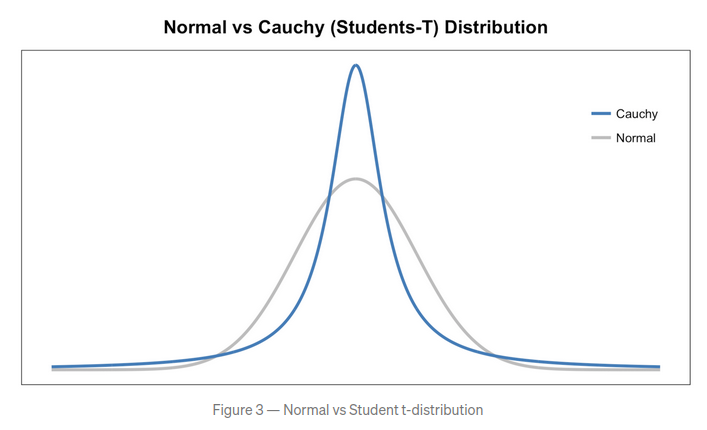
\includegraphics[width=.5\linewidth]{Images/Gaus_vs_Cauchy.png}
  \caption[Cauchy vs Gaussian Distribution]{Cauchy vs Gaussian Distribution. The Cauchy distribution is used in t-SNE to favor small distance similarities.}
  \label{fig:cauchyguas}
\end{figure}
% subsubsection t_distributed_stochastic_neighbor_embedding_ (end)
\newpage
\subsection{Tools} % (fold)
\label{sub:tools}


\subsubsection{Spectrogram and STFT windowing} % (fold)
\label{ssub:spectrogram_and_stft_windowing}
\begin{itemize}
  \item both the raw data (time-resolved) and the spectrogram data (time- and frequency resolved) need to be segmented in windows to be analyzed
  \item \textbf{STFT}
  \begin{itemize}
    \item STFT:
    \begin{equation}
      X(m, \omega) = \sum_{n=-\infty}^\infty x[n]w[n-m]e^{-j\omega n}
    \end{equation}
    $\Longrightarrow$ where w[...] is the window function, most commonly Hann window, x = signal, and $\omega$ is frequency
    \item windowing in STFTs is critical as frequency resolution depends on window length:
    \begin{equation}
      \Delta f = \frac{fs}{n_{samples}}
    \end{equation}
    \item bigger windows lead to better frequency resolution but worse time resolution
    \item a hop length, which defaults to the window length, can be specified to have overlapping windows:
    \begin{equation}
        n_{overlap} = n_{window} - n_{hop}
    \end{equation}
  \end{itemize}
  \item \textbf{Spectrogram Windowing}
  \begin{itemize}
    \item for CNN classifiers, working with spectrograms, the algorithm needs a standardized window length
    \item the windows which are classified are \textbf{context windows} $\Longrightarrow$ \textbf{context window length} is the number of samples used in one context window
    \item each context window will lead to one classification and thus yield one score per class
    \newline \indent $\longrightarrow$ for detectors only one score
    \item hop size is critical for spectrogram classifiers, because units could be cut up by windowing, thus a smaller hop size increases the likelihood of the unit being fully preserved in a window
    \item the context window hop size is thus the number of samples by which a context window is shifted
    \item the context window hop size has to be a multiple of the STFT hop size, as the spectrogram can only be shifted by multiples of the fourier transformed windows
    \item the number of scores resulting from a classification can be calculated:
    \begin{equation}
      n_{scores} = \mathrm{floor}(\frac{n_{signal} - n_{context \, window}}{n_{context \, window \, hop}} +1 )
    \end{equation}
    $\Longrightarrow$ where $n_{context \, window \, hop} = \mathrm{floor}(\frac{n_{context \, window \, hop}}{n_{stft \, hop}}) * n_{stft \, hop}$ 
    \newline \indent $\longrightarrow$ meaning that the context window hop is a multiple of the stft hop \\
    $\Longrightarrow$ the $- n_{context \, window}$ is necessary, as the first context window starts with the context window length and every subsequent context window is shifted by the context window hop
  \end{itemize}
\end{itemize}
% subsubsection spectrogram_and_stft_windowing (end)
\subsubsection{Singular Value Decomposition} % (fold)
\label{ssub:singular_value_decomposition}
\begin{itemize}
  \item SVD can decompose a dataset matrix \textbf{X} into the matrix multiplication of 3 matrices: $U \, \Sigma \, V^T$, with $V = \begin{pmatrix}
    c_1 & c_2 & ... & c_n
  \end{pmatrix} $, where $c_i$ are the principal components
  \item coding example: 
  \begin{python}
    X_centered = X - X.mean(axis=0) 
    U, s, Vt = np.linalg.svd(X_centered)
    c1 = Vt.T[:, 0]
    c2 = Vt.T[:, 1]
  \end{python}
\end{itemize}
% subsubsection singular_value_decomposition (end)

\subsubsection{Self-organizing (feature) map - SOM} % (fold)
\label{ssub:self_organizing_}
\begin{itemize}
  \item unsupervised machine learning technique used to produce a 2D representation of higher order dimensional data while preserving the topological structure.
  \item is trained with competitive learning
  \newline \indent $\longrightarrow$ form of unsupervised learning in ANN's where nodes compete for the right to respond to a subset of the input data
\end{itemize}
% subsubsection self_organizing_ (end)
\subsubsection{Cross Entropy} % (fold)
\label{ssub:cross_entropy}
\begin{itemize}
  \item different functions are used to minimize the cost function
  \item cross-entropy is frequently used to measure how good the match is between a set of estimated class probabilities and the target classes
  \item cross entropy cost function:
  \begin{equation}
    J(\Theta)  = - \frac{1}{m}\sum^m_{i=1} \sum^K_{k=1} y_k^{(i)}\log(\hat p_k^{(i)})
  \end{equation}
  $\Longrightarrow$ $y_k^{(i)}$ is the probability that the ith instance belongs to class k - either 1 or 0 (belongs or doesn't belong)
  \item 
\end{itemize}
% subsubsection cross_entropy (end)
\subsubsection{Data Augmentation} % (fold)
\label{ssub:data_augmentation}
\begin{itemize}
  \item Data Augmentation can be used to generate more training instances from the available data
  \item augmentations should be subtle enough so that a human can't tell the difference between the original and the augmented data
  \item common means of augmentation for images are cropping, rotating, shifting, changing lighting conditions, and any combination of these
  \item it's important, that only augmentations are used that can be learned, so an addition of white noise does not count as augmentation
\end{itemize}
% subsubsection data_augmentation (end)

% subsection tools (end)
\subsection{Precision Metrics in Binary Classification Tasks} % (fold)
\label{sub:precision_metrics_in_binary_classification_tasks}
\begin{itemize}
  \item if class predictions are based on probabilities instead of direct class prediction, thresholds to guide choices can be learned
  \item this allows to set different weights fo \textbf{False Positives} and \textbf{False Negatives} depending on the consequences of such an error
  \item performance measures shown in fig. \ref{fig:roc_pr}
  \item in general: 
  \begin{itemize}
    \item ROC curves should be used when there are roughly equal numbers of observations for each class
    \item PR cuves should be used when there is a moderate to large class imbalance
  \end{itemize}
\end{itemize}
\begin{figure}
  \centering
  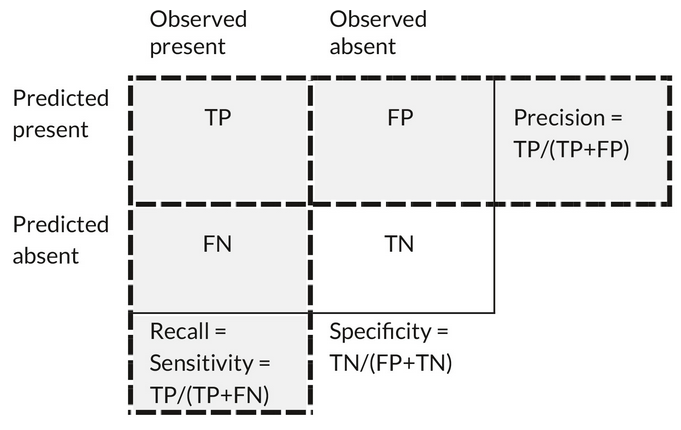
\includegraphics[width=.5\linewidth]{Images/ROC_PR.png}
  \caption[Confusion matrix showing performance measures for ROC and PR]{Confusion matrix showing performance measures for ROC and PR. }
  \label{fig:roc_pr}
\end{figure}

\subsubsection{Receiver Operating Characteristic Curve (ROC)} % (fold)
\label{ssub:receiver_operating_characteristic}
\begin{itemize}
  \item plot of false positives rate (x-axis) versus the true positive rate (\textbf{Sensitivity}) (y-axis) for different threshold values between 0 and 1
  \newline \indent $\longrightarrow$ false alarm vs. hit rate
  \item True pos. rate = TP / (TP + FN)
  \newline \indent $\longrightarrow$ describes how good the model is at predicting the positive class when the actual outcome is positive
  \newline \indent $\hookrightarrow$ also referred to as \textbf{Sensitivity}
  \item False pos. rate = FP / (FP + TN)
  \newline \indent $\longrightarrow$ describes how often a positive is predicted when the actual outcome is negative
  \newline \indent $\hookrightarrow$ also called \textbf{inverted Specificity}
  \item Specificity = TN / (TN + FP)
  \newline \indent $\longrightarrow$ describes how often a negative was predicted when the actual outcome is negative
  \item False pos. rate = 1 - Specificity
  \item Area Under the Curve (AUC) of ROC curve can be used to summarize a models skill
  \newline \indent $\longrightarrow$ \textbf{skill} of a model is the characteristic of assigning a higher probability to a randomly chosen real positive, than a negative on average
  \newline \indent $\hookrightarrow$ skilful models are represented by curves that bow up to the top left of the plot
  \item a model with no skill is represented at the center point (0.5, 0.5)
  \item a model with no skill at every threshold is represented by a diagonal line from the bottom left of the plot to the top right and has a AUC of 0.5
  \item a model with perfect skill is represented at point (0, 1)
  \item a model with perfect skill at every threshold is represented by a vertical line from the bottom left to the top left and then a horizontal line to the top right (AUC = 1)
\end{itemize}
% subsubsection receiver_operating_characteristic_ (end)

\subsubsection{Precision-Recall Curve (PR)} % (fold)
\label{ssub:precision_recall_curve_}
\begin{itemize}
  \item plot of the \textbf{Precision} (y-axis) and \textbf{Recall} (x-axis) for different thresholds
  \item Precision = TP / (TP + FN)
  \newline \indent $\longrightarrow$ describes how good a model is at predicting the positive class
  \newline \indent $\hookrightarrow$ also referred to as the positive predictive value 
  \item Recall = TP / (TP + FN) ( = Sensitivity)
  \item PR curves are useful in cases where there are many examples of no event and only a few examples of an event
  \item PR curves don't care about TN, because they are only interested in positives (in the minority class)
  \item a model with no skill and varying threshold is represented by a horizontal line, the hight depends on the class balance of the data
  \item a model with perfect skill is represented at the point (1, 1)
  \item a skilful model is represented by a curve that bows towards (1, 1) above the flat line of no skill
  \item PR curves can be evaluated with the \textbf{F-Measure}: harmonic mean of precision and recall rates, and AUC
  \item F-Measure summarizes skill for a specific threshold value
  \item AUC summarizes the skill of amodel across thresholds
\end{itemize}
% subsubsection precision_recall_curve_ (end)
% subsubsection precision_metrics_in_binary_classification_tasks (end)



\subsection{Deep Neural Networks} % (fold)
\label{sub:deep_neural_networks}

\subsubsection{Basic Structure} % (fold)
\label{ssub:basic_structure}
\begin{itemize}
  \item from  \cite{geron_hands-machine_2019} (Chapter 10)
  \item Deep Neural Networks are ANN's with a of deep stack hidden layers  
  \begin{itemize}
    \item ANN (artificial neural networks) first comprised of Perceptron (invented in 1957)
    \newline \indent $\longrightarrow$ based on an artificial neuron called threshold logic unit (TLU):
    \begin{itemize}
      \item inputs with weights are computed into a weighted sum, then step function is applied outputting: $h_w(x) = \mathrm{step}(z)$, while $z = x^T w$, w = weights, x = inputs
      \item common step functions are sign function (-1 if z<0, 0 if z = 0, 1 if z > 0) or heavyside (0 if z<0, 1 otherwise)
      \item TLU can be used for simple linear binary classification (just like Logistic Regression classifier or linear SVM)
    \end{itemize}
    \item a Perceptron is composed of a single layer of TLUs, all TLUs are connected to all inputs
    \newline \indent $\longrightarrow$ if all neurons in a layer are connected to eveery neuron in the previous layer (i.e., the inputs) it's called a \textbf{dense layer}.
    \newline \indent $\hookrightarrow$ for consistence, usually input neurons are drawn, just outputting whatever input they are fed
    \newline \indent $\longrightarrow$ a bias feature is generally added ($x_0=1$) it's typically represented using a special type of neural called bias neuron, outputting 1 all the time - so to say the first input
    \item a 2 input - 3 output perceptron is shown in \ref{fig:perceptron}
    \item calculating the outputs:
    \begin{equation}
      h_{W, b} = \Phi (XW + b)
    \end{equation}
    \begin{itemize}
      \item W - weight matrix: all weights except for bias
      \item b - bias vector: all connection weights between bias neuron and artificial neurons
      \item X - input matrix
      \item $\Phi$ - activation function
    \end{itemize}
    \item "Cells that fire together, wire together." - Hebbian learning
    \newline \indent $\longrightarrow$ connection weight between two neurons is increased when output is same
    \item perceptrons are trained so that after a training instance is run and a prediction is made, for every output neuron producing a incorrect prediction, the connection weights from the inputs that would have yielded the correct predictions are strengthened
    \begin{equation}
      w_{i, j}^{\text{(next step)}} = w_{i, j} + \eta(y_j - \hat y_j) x_i
    \end{equation}
    \begin{itemize}
      \item $w_{i, j}$ - connection weight between ith neuron and jth output neuron
      \item $x_i$ - ith input value
      \item $\hat y_j$ - output of jth output neuron
      \item $y_j$ - target output of jth ourput neuron
      \item $\eta$ - learning rate
    \end{itemize}
    \item all decision boundaries from output neurons are linear in perceptrons, making them incapable of learning complex patterns (like Logistic Regression classifiers)
    \newline \indent $\longrightarrow$ if training instances are linearly separable, the algorithm would converge to a solution
    \item Perceptron learning algorithm is equivalent to \textbf{Stochastic Gradient Descent} with no penalty (no regularization) and constant learning rate
    \newline \indent $\hookrightarrow$ SGD - picks random training points to not use every training point, so it's good for large training sets (it's important that the training instances are truly chosen at random! - otherwise only one class gets learned before the next class is introduced) 
    \newline \indent $\longrightarrow$ perceptrons give out hart class predictions, they don't provide probabilities for classes like Logistic Regression classifiers
    \item to be able to solve a XOR, which is not possible with standard perceptron logic, a MLP (multi-layer perceptron) needs to be used, adding an extra layer - a hidden layer
    \item lower layers are close to input, upper layers are close to output
    \newline \indent $\longrightarrow$ every layer except for the output layer has a bias neuron and is fully connected to the next layer
  \end{itemize}
  \item to train MLP's backpropagation was instroduced
  \newline \indent $\longrightarrow$ for every training instance the networks is run through forwards and backwards (happens in parallel)
  \newline \indent $\hookrightarrow$ one iteration of the entire training set is an \textbf{epoch}
  \item on the backwards pass, the network calculates the loss-function comparing the desired output values with the actual output values, returning a measure of error
  \newline \indent $\longrightarrow$ it then works its way back to the input computing how much each output contributed to the error
  \newline \indent $\hookrightarrow$ once the errors are all calculated, a Gradient Descent is performed for every weight in the network
  \item backpropagation relies on unsymmetric weights, that's why randomly initializing the weights is crucial
  \item for Gradient Descent to properly work, a continuous function was needed, introducting the \textbf{logistic function}: $\sigma(z) = 1/(1 + e^{-z})$
  \newline \indent $\longrightarrow$ other famous activation functions are: 
  \begin{itemize}
    \item \textbf{hyperbolic tangent function}: $\tanh(z)~=~2\sigma(2z)~-~1$
    \newline \indent $\longrightarrow$ goes from -1 to 1, unlike $\sigma$ (from 0 to 1), can speed up convergence as values center around 0
    \item \textbf{Rectified Linear Unit functio}n: $\mathrm{ReLU}(z) = \mathrm{max}(0, z)$
    \newline \indent $\longrightarrow$ not differentiable at z=0, very fast to compute, doesn't have a max wich can be advantageous
  \end{itemize}
  \item why are activation functions needed in the first place?
  \newline \indent $\longrightarrow$ if no activation functions are used, all weights are just chained, leading to only linear functions ($f(x) = 2x+3 \text{ and } g(x) = 3x -3 \Longrightarrow f(g(x)) = 2(3x-3) + 3 $), so activation functions introduce the non-linearity enabling us to solve non-linear boundaries between classes
  \item depending on the output of the NN, it can be good to have a activation function in the output layer, limiting values
  \item error functions to use:
  \begin{itemize}
    \item typically: mean squared error
    \item in case of many outliers: mean absolute error
    \item alternatively: Huber loss, which combines both: quadratic when error is smaller than threshold (mostly 1) and linear when larger
    \newline \indent $\longrightarrow$ less sensitive to outliers whilst more accurate and faster in converging than mean absolute error
  \end{itemize}
  \item standard MLP classification setup: \cite{geron_hands-machine_2019} page 291
  \item MLP vs CNN vs RNN
  \begin{itemize}
    \item MLP: vectors as inputs
    \item CNN: tensor as input, is able to understand spatial resolution, thus better for complex images
    \item RNN: designed to work for problems related to sequence like sequence of words in sentences, or sounds in speech recognition
  \end{itemize}
\end{itemize}

\begin{figure}
  \centering
  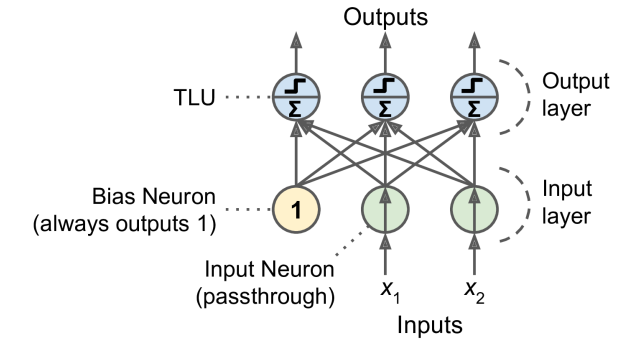
\includegraphics[width=.5\linewidth]{Images/perceptron.png}
  \caption[Perceptron structure]{Perceptron structure. structure of a simple perceptron with 2 inputs and 3 outputs.}
  \label{fig:perceptron}
\end{figure}

\subsubsection{Long Short-Term Memory network (LSTM)} % (fold)
\label{ssub:long_short_term_memory_network_}
\begin{itemize}
  \item advanced RNN (sequential network), that allows information to persist
  \newline \indent $\longrightarrow$ can learn in what way sequences are relevant
  \newline \indent $\longrightarrow$ can handle vanishing gradient problem
  \item RNNs can remember short sequences, but with longer sequences, they can't because of vanishing gradients, LSTMs are designed to also remember long sequences
\end{itemize}
% subsubsection long_short_term_memory_network_ (end)


\subsubsection{Intuition for NN structure} % (fold)
\label{ssub:intuition_for_nn_structure}
\begin{itemize}
  \item the book \cite{geron_hands-machine_2019} led me to the website \url{www.playground.tensorflow.org}, which is ideal to play around and get a good intuition for neural network structures
  \item when choosing the spiral data, the only activation function that works well is tanh, simply because all other functions work on a linear basis
  \item all input properties are required to sufficiently approximate the complex shape of a spiral
  \item at least 3 hidden layers, rather 4 are needed to sufficiently approximate the spiral
  \item more neurons, which are the analogon to feature maps, take more computational power but are able to approach the spiral far faster than having only 2 or 3 neurons per hidden layer
  \item a set up of 4 hidden layers and 6 neurons each yields a very good loss value after less than 200 epochs
  \item the tool shows, that similar results can be reached with different network structures taking different amount of computational time
\end{itemize}
% subsubsection intuition_for_nn_structure (end)

\subsubsection{Challenges of Training Deep Neural Networks} % (fold)
\label{ssub:challenges_of_training_deep_neural_networks}
\begin{itemize}
  \item \textbf{vanishing gradients} - gradients often get smaller and smallers as the algorithm progresses down to the lower layers, resulting in the Gradient Descent update leaving the lower layer connection weights almost unchanged
  \item \textbf{exploding gradients} - in RNN (recurrent neural networks) this problem can arise causing diverging results
  \item the main driver is the logistic activation function, which saturates for very high values (also negative) and results in very small gradients
  \newline \indent $\longrightarrow$ these then cascade down and there is little gradient left to change low layer weights 
  \item randomly initializing the weights in the beginning can fight this issue
  \item choice of activation function also plays a bis role for the vanishing gradients - ReLU performs better than logistic activation function, however the gradient for negative values is 0, thus if in a cascade neurons are connected that all have negative values, the wont learn anymore
  \item scaled exponential linear unit (SELU) is a activation function that approaches -1 for negative values and $\alpha$ for positive values, wich $\alpha$ being a hyperparameter
  \newline \indent $\longrightarrow$ though this takes longer, it avoids both the dead neuron and the vanishing gradients problem making it a very good activation function for many problems
  \newline \indent $\longrightarrow$ when used, the initialization of the weights has to be LeCun normalization: kernel\_initializer="lecun\_normal"
  \newline \indent $\longrightarrow$ network needs to be sequential, otherwise self-normalization is not guaranteed and the SELU might be worse than others
  \item in general SELU > ELU (similar to SELU but z(0) = 0) > leaky ReLU ($\alpha = 0.3$ is keras' standard, but it can be changed) > ReLU > tanh > logistic
  \newline \indent $\longrightarrow$ if SELU not possible, then ELU
  \begin{python}
    # for leaky ReLU:
    leaky_relu = keras.layers.LeakyReLU(alpha = 0.2)
    layer = keras.layers.Dense(10, activation = leaky_relu,
                                kernel_initializer = "he_normal")

    # for SELU:
    layer = keras.layers.Dense(10, activation="selu",
                                kernel_initializer="lecun_normal")
  \end{python}

\end{itemize}

\subsubsection{Optimizations} % (fold)
\label{ssub:optimizations}

\begin{itemize} 
  \item \textbf{Batch Normalization} - used to zero-center and normalize each input just so that they can be shifted and scaled thereafter, but the shifting and scaling is learnable
  \newline \indent $\longrightarrow$ BN is so powerful, that it vastly reduces number of epochs, acts as a regularization (fighting overfitting) and allows the usage of saturating activation functions (tanh, even logistic)
  \newline \indent $\longrightarrow$ each epoch will take longer, but convergence will be reached far sooner than without BN
  \begin{python}
    model = keras.models.Sequential([
        keras.layers.Flatten(input_shape=[28, 28]),
        keras.layers.BatchNormalization(),
        keras.layers.Dense(300, activation="elu", 
                          kernel_initializer="he_normal"),
        keras.layers.BatchNormalization(),
        keras.layers.Dense(100, activation="elu", 
                          kernel_initializer="he_normal"),
        keras.layers.BatchNormalization(),
        keras.layers.Dense(10, activation="softmax")
        ])
  \end{python}
  \item the batch normlalization is computed by calculating the mean and standard deviation of every input, or every batch, there are several parameters than get learned in the BN, due to the rescaling and shifting
  \newline \indent $\longrightarrow$ additionally there are hyperparameters, momentum (used when updating moving averages; usually close to 1) and axis (dictates which axis should be normalized; defaults to -1), which get tweaked on a global level
  \newline \indent $\hookrightarrow$ axis can also be list, if pixels should be treated independently: axis = [1, 2] 
  \item \textbf{Optimizers} - optimizers help speed up the learning by realizing if they are on a plateau or in a valley and accelerate learning rate or other hyperparameters to speed up the search for the global minimum
  \item most common: adaptive moment estimation (ADAM) combines benefits of momenum optimization and RMSProp
  \newline \indent $\longrightarrow$ in general Adam > RMSProp > Nesterov Accelerated Gradient > Gradient Descent
  \newline \indent $\hookrightarrow$ if model performs bad try Nesterov Accelerated Gradient instead of Adam, the data might not like adaptive momentum optimizers, but in general they are the best (currently) 
  \item it might be advantageous to use a learning rate scheduler, to make use of large learning rates at first and then reduce it to slow down
\end{itemize}
% subsubsection optimizations (end)


% subsubsection challenges_of_training_deep_neural_networks (end)

% subsection deep_neural_networks (end)
\subsection{Convolutional Neural Networks (CNN)} % (fold)
\label{sub:convolutional_neural_networks_}

\subsubsection{History and Concept} % (fold)
\label{ssub:history_and_concept}

% subsubsection history_and_concept (end)
\begin{itemize}
  \item summary of \cite{geron_hands-machine_2019} chapter 14
  \item CNNs were invented following new findings about the human visual perctive system, showing that different neurons wihtin an area of the receptive field recognize different patters - i.e., some horizontal lines, some vertical lines, some round shapes ...
  \item using conventional MLPs for complex image recognition leads to a huge number of weights very fast, so CNN was introduced using alternative concepts to avoid millions of weights
  \item led to invention of the neocognitron, which is now called CNN
  \item CNNs use fully connected layers (dense layers) and sigmoid activation functions, additionally they use convolutional layers and pooling layers
  \begin{itemize}
    \item \textbf{convolutional layer}: neurons are not connected to every pixel (input) neuron, but rather only to pixels in the receptive field
    \newline \indent $\longrightarrow$ this allows to focus on low-level features on the first hidden layer, then assemble those together to get higher-level features etc, see \ref{fig:conv_lay}
    \item layers are now 2d grids, rather than flat 1d vectors
    \item usually zeros are padded to the smaller layers, to maintain the same size
    \item the overlap step size between the layers is called a \textit{stride} - stride = 1 dimensionality reduction of -1 in both dimensions, stride = 2 $\Longrightarrow$ -2 ...
  \end{itemize}
  \item \textbf{filters} can be used to bias the algorithm in a certain direction
  \begin{itemize}
    \item while converging a square of pixels is reduced to a single value, if this square has a inherent weighting of all 0s and only 1s in one line, the resulting layer will filter for horizontal images, see \ref{fig:filter}
    \item the filters get optimized automatically, causing certain patterns to be far more prominent than others
  \end{itemize}
\end{itemize}
\begin{figure}
  \centering
  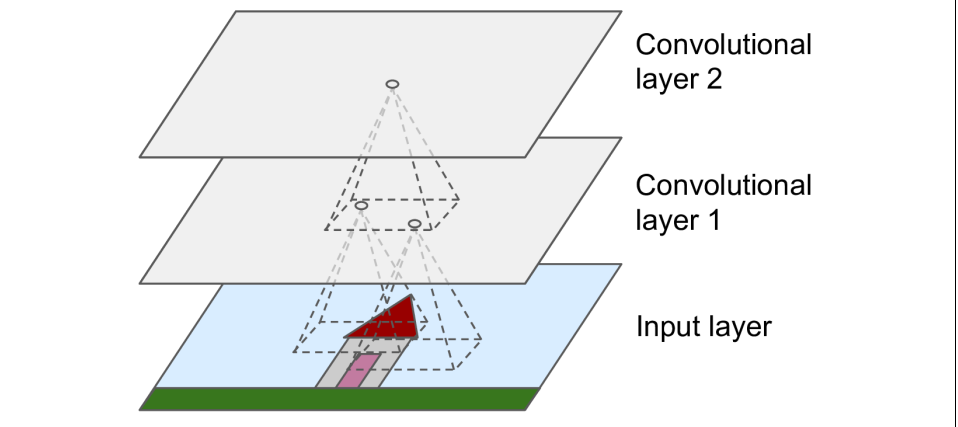
\includegraphics[width=.5\linewidth]{Images/convolutional_layer.png}
  \caption[Convolutional Layer]{Convolutional Layer. Convolutional layers don't connect every neuron to every neuron of the lext layer, but rather group the converging process, thus reducing the number of weights, whilst promoting patterns in a specific area.}
  \label{fig:conv_lay}
\end{figure}

\begin{figure}
  \centering
  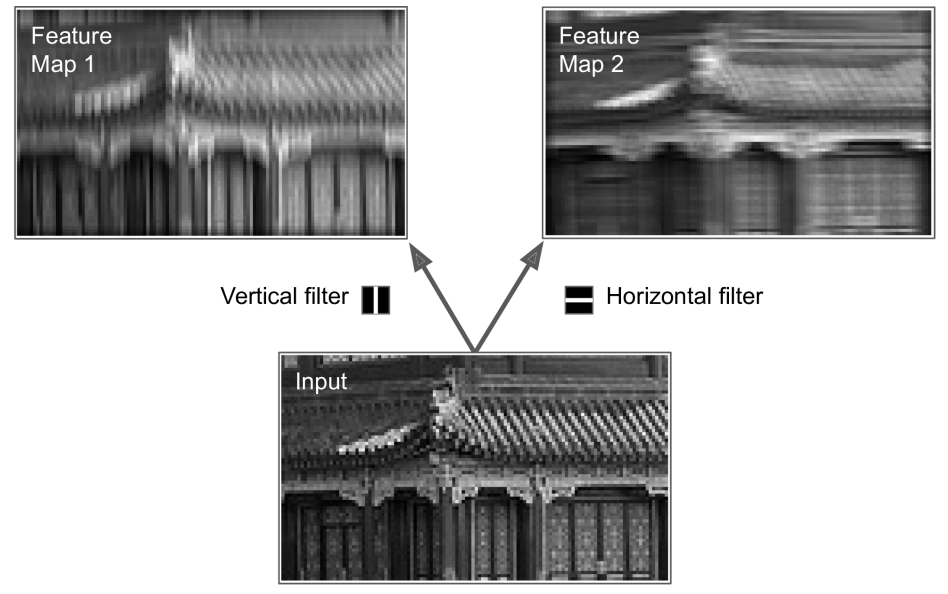
\includegraphics[width=.5\linewidth]{Images/filter.png}
  \caption[Filter applied between convolutional layers]{Filter applied between convolutional layers. The inherent weighting in the converging square shapes the bias of the next layer.}
  \label{fig:filter}
\end{figure}

\begin{itemize}
  \item the number of filters is not limited to one, usually convolutional layers have multiple filters and output multiple feature maps - one per filter
  \item so for one are of pixels different filters are applied, allowing the layer to detect different patterns in the same area
  \newline \indent $\longrightarrow$ the subsequent layer will have the same convergence, leading to pattern recognition on the already abstracted previous feature map - this way small and large scale patterns can be learned
  \item neurons of one feature map all have the same parameters: weights and bias term $\Longrightarrow$ this dramatically reduces the number of parameters in the model
  \newline \indent $\longrightarrow$ this way a pattern in one location will also be recognized in another location
  \item the equation used to compute the output of a neuron in a conv layer:
  \begin{align}
    z_{i, j, k} = &bias_{FeatMap} + \sum^{height-1}_{row=0} \sum^{width-1}_{col=0} \sum^{FeatMapsInPrevLayer-1}_{PrevFeatMap=0}&&  \nonumber \\ 
    &x_{(i\cdot stride_{row} + row), \,(j\cdot stride_{col} + col), \,PrevFeatMap} \, \cdot  \, w_{row, \,col, \, PrevFeatMap, \,FeatMap} &&
  \end{align}
  \newline \indent $\longrightarrow$ x is output neuron in layer l-1 (in ($i\cdot stride_{row} + row, \,j\cdot stride_{col} + col$) and PrevFeatMap)
  \newline \indent $\longrightarrow$ w is the connection weight between neuron of layer l and its input (in (row, col) and FeatMap) 
  \newline \indent $\longrightarrow$ z is the output of neuron (in (i, j) and FeatMap)
\end{itemize}
\subsubsection{Implementation in TensorFlow} % (fold)
\label{ssub:implementation_in_tensorflow}

% subsubsection implementation_in_tensorflow (end)

\begin{itemize}
  \item input images are represented as 3D tensor - [height, width, channels]
  \newline \indent $\longrightarrow$ mini-batch is thus a 4D tensor - [mini-batch size, height, width, channels]
  \newline \indent $\longrightarrow$ layers of convolutional layer also 4D tensor - [height, width, FeatMapsInPrevLayer, FeatMapInCurrentLayer]
  \newline \indent $\longrightarrow$ bias terms of convolutional layers are 1D tensor - [FeatMapInCurrentLayer]
  \item Implementation in tensorflow using 2 images with 256 depth per pixel:

  \begin{python}
  from sklearn.datasets import load_sample_image
  
  # Load sample images
  china = load_sample_image("china.jpg") / 255
  flower = load_sample_image("flower.jpg") / 255
  
  images = np.array([china, flower])
  batch_size, height, width, channels = images.shape
  
  # Create 2 filters
  filters = np.zeros(shape=(7, 7, channels, 2), dtype=np.float32)
  filters[:, 3, :, 0] = 1 # vertical line
  filters[3, :, :, 1] = 1 # horizontal line
  
  outputs = tf.nn.conv2d(images, filters, strides=1, padding="SAME")
  plt.imshow(outputs[0, :, :, 1], cmap="gray") # plot 1st image's 2nd feature map
  plt.show()
  \end{python}
  \indent $\longrightarrow$ mini-batch size is 2 in this case, as we have 2 images
  \newline \indent $\longrightarrow$ padding = 'SAME' - zero padding is used when necessary. number of output neurons = ceil( number of input neurons / stride )
  \newline \indent $\hookrightarrow$ alternatively padding = 'VALID' - zero padding is not used by convolutionaly layer, this may lead to it ignoring some rows and columns
  \item filters were fixed here, but usually filters would be trainable variables. this can all be done in one step:
  \begin{python}
     conv = keras.layers.Conv2D(filters = 32, kernel_size = 3, strides = 1, padding ='SAME', activation = 'relu')
   \end{python} 
   \indent $\longrightarrow$ this creates a Conv2D layer with32 filters, each 3x3, stride of 1, SAME padding and RELU activation function
   \item as there are already a lot of choices for hyperparameters in CNN layers, cross-validation can be helpful to find optimal parameters, which is however, very time consuming
   \item During a training session, all weights need to be stored in memory, ready to be updated when the backpropagation happens, as a result, the amount of memory (RAM) required is NumOfFeatureMaps x HeightOfFeatureMap x WidthOfFeatureMap x DepthOfFloats x NumOfInstances
   \newline \indent $\longrightarrow$ so 200 x 150 x 100 x 32 x 100 = 1.2 GB (200 features maps with size 150 x 100, 32-bit floats, 100 instances) - can get large very quickly
   \item Out of Memory Errors can be handled by higher strides, removing some layers, 16-bit floats instead of 32
\end{itemize}

\subsubsection{Pooling layers} % (fold)
\label{ssub:pooling_layers}

% subsubsection pooling_layers (end)
\begin{itemize}
  \item pooling layers shrink or subsample the input image, thus converging an array to a single value
  \newline \indent $\longrightarrow$ the idea is obviously a reduction in computational load and memory usage - ideally leading to a lower risk of overfitting
  \item instead of having a filter that applies a weighting scheme but preserves the size of the input image and feature map, the pooling layer aggregates all pixel values and combines them into one values
  \newline \indent $\longrightarrow$ this combination can be based on functions like max or mean - i.e. \textit{max pooling layer}
  \item max pooling layers can be advantageous as they have a certain invariance. The max value in a square or rectangle might remain the same even if the image is slightly rotated or the scale is slightly different
  \newline \indent $\longrightarrow$ for classification tasks this can be crucial as not to miss patterns due to slightly different angles of a shot or different scale
  \newline \indent $\hookrightarrow$ not so much relevant for spectrograms, as dimensions and freq resolution is always the same
  \item this invariance is of course also an information loss and can be a problem, all depends on the task at hand
  \begin{python}
    max_pool = keras.layers.MaxPool2D(pool_size = 2)
  \end{python}
  $\Longrightarrow$ this will create a max pooling layer with a 2x2 kernel and a stride of 2 (defaults to kernel size) and VALID padding
  \item AvgPool2D would create a average pooling layer, however usually the most prominent pixel should be preserved, resulting in max pooling layers being far more commonly used
  \item pooling layers can also be used to learn depth-wise, for example different filters in the convolutional layers apply different rotations and then the pooling layer identifies the filter that best identifies the feature, see fig. \ref{fig:pool-depth}
  \item to use a depth-wise pooling layer, do:
  \begin{python}
    output = tf.nn.max_pool(images, 
                            ksize = (1, 1, 1, 3), 
                            strides = (1, 1, 1, 3), 
                            padding = 'VALID')
  \end{python}
  $\Longrightarrow$ the (1, 1, 1, 3) indicates that the kernel size and stride along the batch, height and width sould be 1. the last digit defines the kernel size and stride along the depth dimension (must be a divisor of the input depth/number of previous feature maps)
  \item to include it in Keras models, you can wrap it in a Lambda layer (or create a custom Keras layer):
  \begin{python}
    depth_pool = keras.layers.Lambda( lambda X: tf.nn.max_pool(X, 
                                          ksize = (1, 1, 1, 3), 
                                          strides = (1, 1, 1, 3), 
                                          padding = 'VALID') )
  \end{python}
  \item \textit{global average pooling} layer is common nowadays - computes the mean of entire feature map into one value
  \begin{python}
    global_avg_pool = keras.layers.GlobalAvgPool2D()
    global_avg_pool = keras.layers.Lambda( lambda X: tf.reduce_mean(X, 
                                          axis=[1, 2]) ) 
    # the second one does the same as the above
  \end{python}
\end{itemize}
\begin{figure}
  \centering
  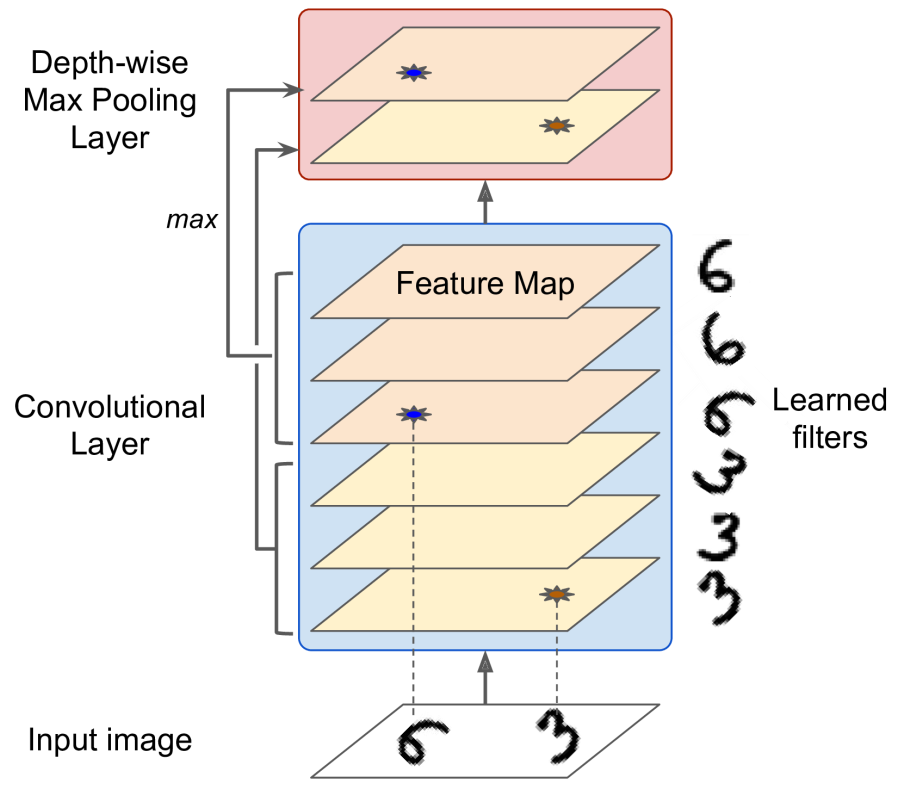
\includegraphics[width=.5\linewidth]{Images/depth-pooling.png}
  \caption[CNN learning hand written images with pooling along depth-dimension]{CNN learning hand written images with pooling along depth-dimension. Convulutional layers are used to filter for different rotations of hand written digits and then pooling layers are used to find the rotations best preserving the feature.}
  \label{fig:pool-depth}
\end{figure}

\subsubsection{CNN Architectures} % (fold)
\label{ssub:cnn_architectures}
\begin{itemize}
  \item typically CNNs are comprised of a few convolutional layers (in addition to a subsequent ReLU layer) then a pooling layer, more convolutional layers ( + ReLU), then another pooling layer and so forth
  \newline \indent $\longrightarrow$ image gets smaller due to pooling
  \newline \indent $\longrightarrow$ number of feature maps increases, image gets \textit{deeper} resulting from convolutional layers
  \newline \indent $\hookrightarrow$ finally, a regular feedforward neural network comprised of fully connected layers (+ReLU) and a final layer output a prediction (or class probabilities using for example a softmax (function to draw boundaries between classes) layer)
  \item convolutional kernels that are too large can be problematic, use two stacked layers with 3x3 kernels rather than one 5x5 kernel
  \newline \indent $\longrightarrow$ less parameters and less computations required
  \newline \indent $\hookrightarrow$ exception: initial layer: 5x5 and stride = 2 is good for first layer - decreases dimension but loss is not to heavy (might not apply for spectrograms)
  \item example implementation for a MNIST dataset:
  \begin{python}
    from functools import partial
    
    DefaultConv2D = partial(keras.layers.Conv2D,
                            kernel_size=3, 
                            activation='relu', 
                            padding="SAME")

    model = keras.models.Sequential([
            DefaultConv2D(filters=64, kernel_size=7, 
                          input_shape=[28, 28, 1]),
            keras.layers.MaxPooling2D(pool_size=2),
            DefaultConv2D(filters=128),
            DefaultConv2D(filters=128),
            keras.layers.MaxPooling2D(pool_size=2),
            DefaultConv2D(filters=256),
            DefaultConv2D(filters=256),
            keras.layers.MaxPooling2D(pool_size=2),
            keras.layers.Flatten(),
            keras.layers.Dense(units=128, activation='relu'),
            keras.layers.Dropout(0.5),
            keras.layers.Dense(units=64, activation='relu'),
            keras.layers.Dropout(0.5),
            keras.layers.Dense(units=10, activation='softmax'),
    ])
  \end{python}
  $\Longrightarrow$ the partial in the beginning allows us to define a default that doesn't need to be repeated over and over
  \newline \indent $\longrightarrow$ with input image size of 28x28 and grayscale, a stride of 7 with no stride because images are not that large
  \newline \indent $\longrightarrow$ pooling layer, reducing the spatial dimension by factor of 2
  \newline \indent $\longrightarrow$ repeat the structure of 2 conv layers and one pooling layer
  \newline \indent $\hookrightarrow$ depending on input image size this process can be repeated more than twice
  \newline \indent $\longrightarrow$ doubling of filters after pooling layers (which reduce spatial dimensions by factor 2) is common, as number of higher level features (embedded deeper into image, only get revealed after a lot of pooling) is bigger than lower level features
  \newline \indent $\longrightarrow$ finally the fully connected network, made of 2 hidden layers and dense output layer. inputs must be flattened because dense networks expect 1D arrays
  \newline \indent $\hookrightarrow$ the Dropout layers with a dropout rate of 50 \% are used to reduce overfitting
  \item this is not state of the art but it is a good network, reaching 92 \% accuracy on a MNIST fashion dataset
  \item ILSVRC ImageNet challenge is a good measure of keeping up to date with new networks, in the last 5 years major improvements in the winning networks have been achieved, being able to differentiate between 120 dogbreeds for example
\end{itemize}
% subsubsection cnn_architectures (end)
\subsubsection{LeNet-5} % (fold)
\label{ssub:lenet_5}
\begin{itemize}
  \item most widely known CNN architecture
  \item used for MNIST handwritten digits
  \item structure see table \ref{tab:lenet5}
  \item Avg Pooling used instead of max pooling - each neuron computes the mean of its inputs, multiplies the result by a leanable coefficient (one per map) and adds a trainable bias term (also 1 per map) and then applies activation function
  \item Out layer computes the matrix multiplication of inputs and wight vector, each neuron outputs the square of the distance between its input vector and its weight vector - the output then measures how much the image belongs to a particular digit class
  \newline \indent $\longrightarrow$ cross entropy (sec \ref{ssub:cross_entropy}) preferred as a cost function as it penalizes bad predictions much more, yielding larger gradients and converging faster
\end{itemize}

\begin{table}
  \centering
    \begin{tabular}{|l|l|l|l|l|l|l|}
      \hline
      Layer &Type  &Maps  &Size  &Kernel size  &Stride  &Activation  \\
      \hline
      Out &Dense & - & 10 & - & - & RBF \\
      F6 & Dense &- &84 & - &- &tanh \\
      C5 & Convolution & 120 & 1x1 & 5x5 & 1 & tanh \\
      S4 & Avg Pooling & 16 & 5x5 & 2x2 & 2 & tanh \\
      C3 & Convolution & 16 & 10x10 & 5x5 & 1 & tanh \\
      S2 & Avg Pooling & 6 & 14x14 & 2x2 & 2 & tanh \\
      C1 & Convolution & 6 & 28x28 & 5x5 & 1 & tanh \\
      In & Input & 1 & 32x32 & - &- &-\\  
      \hline
    \end{tabular}
  \caption[Architecture of LeNet-5]{Architecture of LeNet-5. With increasing layer number, maps increase and size decreases resulting from the pooling layers.}
  \label{tab:lenet5}
\end{table}
% subsubsection lenet_5 (end)

\subsubsection{AlexNet} % (fold)
\label{ssub:alexnet}
\begin{itemize}
  \item won the ILSVRC challenge by large margin
  \item was the first to stack convolutional layers directly
  \item table \ref{tab:alexnet} shows the architecture
  \item AlexNet uses local response normalizaion (LRN) after C1 and C3 
  \newline \indent $\longrightarrow$ the most strongly activated neurons inhibit other neurons in the same position but neighboring faeture maps, ths forcing them to explore a wider range of features, improving generalization
  \begin{equation}
    b_i = a_i (k + \alpha \sum^{j_{high}}_{j = j_{low}} a_j^2)^{-\beta} \quad \text{with} 
    \begin{cases}
      j_{high} = \min(i + \frac{r}{2}, f_n -1)\\
      j_{low}  = \max(0, i - \frac{r}{2})
    \end{cases}
  \end{equation}
  \newline \indent $\longrightarrow$ $b_i$ - normalized output of neuron located in feature map i, at some position
  \newline \indent $\longrightarrow$ $a_i$ - activation of that neuron after ReLU before normalization
  \newline \indent $\longrightarrow$ $k, \alpha, \beta, r$ - hyperparameters, with k = bias, r = depth radius
  \newline \indent $\longrightarrow$ $f_n$ is the number of feature maps
  \item if r=2 and a neuron has a strong activation, the neurons in similar positions and neighboring feature maps will be inhibited
  \item for AlexNet: $r = 2, \alpha = 0.00002, \beta = 0.75, k=1$
  \newline \indent $\longrightarrow$ can be altered with 
  \begin{python}
    tf.nn.local_response_normalization()
  \end{python}
\end{itemize}
\begin{table}
  \centering
    \begin{tabular}{|l|l|l|l|l|l|l|l|}
      \hline
      Layer &Type &Maps &Size&Kernel size & Stride &Padding &Activation  \\
      \hline
      Out &Dense &- &1000 &-  & - &- &Softmax  \\
      F9 &Dense & - & 4096 &- &- &- &ReLU \\
      F8 & Dense & - & 4096 &- &- &- &ReLU \\
      C7 & Convolution & 256 & 13x13 & 3x3 & 1 & SAME & ReLU \\
      C6 & Convolution & 384 & 13x13 & 3x3 & 1 & SAME & ReLU \\
      C5 & Convolution & 384 & 13x13 & 3x3 & 1 & SAME & ReLU \\
      S4 & Max Pooling & 256 & 13x13 & 3x3 & 2 & VALID & -   \\
      C3 & Convolution & 256 & 27x27 & 5x5 & 1 & SAME & ReLU \\
      S2 & Max Pooling & 96  & 27x27 & 3x3 & 2 & VALID & - \\
      C1 & Convolution & 96  & 55x55 & 11x11 & 4 & VALID & ReLU \\
      In & Input       & 3 (RGB) & 227x227  &- &- &- &- \\
      \hline
    \end{tabular}
  \caption[Architecture of AlexNet]{Architecture of AlexNet. Much larger than the LeNet-5, and the first to stack convolutional layers.}
  \label{tab:alexnet}
\end{table}
% subsubsection alexnet (end)

\subsubsection{GoogLeNet} % (fold)
\label{ssub:googlenet}
\begin{itemize}
  \item uses \textit{inception modules} allowing it to vastly reduce number of parameters
  \begin{itemize}
    \item inception modules employ different layer combinations that are used in parallel and concatenated in the end (using tf.concat(axis=3 (depth)) )
    \item different kernel sizes are used and combined, also 1x1 kernels are used, that don't reduce in spatial dimensions but rather in depth dimensions, outputting fewer feature maps than were inputted
    \item fig. \ref{fig:inception_module} shows an inception module
    \item every inception layer requires 6 hyperparameters - the kernel sizes of the respective convolutional layers and the max pooling layer
  \end{itemize}
  \item fig \ref{ssub:googlenet} shows the GoogLeNet architecture
  \item first the image is reduced in size by the first two layers 
  \newline \indent $\longrightarrow$ a LRN is used to learn a variety of features 
  \newline \indent $\longrightarrow$ a convolutional network acts as a bottleneck layer - reducing dimensionality (and thus parameters) 
  \newline \indent $\longrightarrow$ another LRN 
  \newline \indent $\longrightarrow$ max pooling, reduces spatial dimensions 
  \newline \indent $\longrightarrow$ a stack of nine inception layers with some max pooling in between to reduce dimensions and speed up the net 
  \newline \indent $\longrightarrow$ global avg pooling gives average of entire feature map (stripping any spatial dimension) 
  \newline \indent $\longrightarrow$ dropout for regularization, fully connected with 1000 units (1000 classes) and softmax activation to get class probabilities
  \newline \indent $\hookrightarrow$ the global average pooling layer can be used, seeing that not much spatial information was left after the 5 fold dimensionality reduction, and location is not of interest, so the crucial information is, does this feature exist or not - which is a lot quicker with just one values per feature map
  \item the massive decrease in spatial information vastly sped up the process, as the final dense layers where only one dimensional (compared to AlexNet where the dense layers were huge) 
\end{itemize}

\begin{figure}
  \centering
  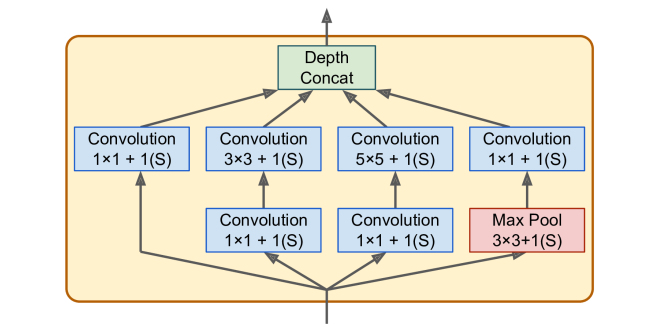
\includegraphics[width=.5\linewidth]{Images/inception_module.png}
  \caption[Inception Module]{Inception Module. Inception module used for example in GoogLeNet. '3x3 + 1(s)' means 3x3 kernel, stride of 1, and same padding. Because stride is 1 everywhere the results have the same spatial dimensions and can be concatenated in the final step.}
  \label{fig:inception_module}
\end{figure}
\begin{figure}
  \centering  
  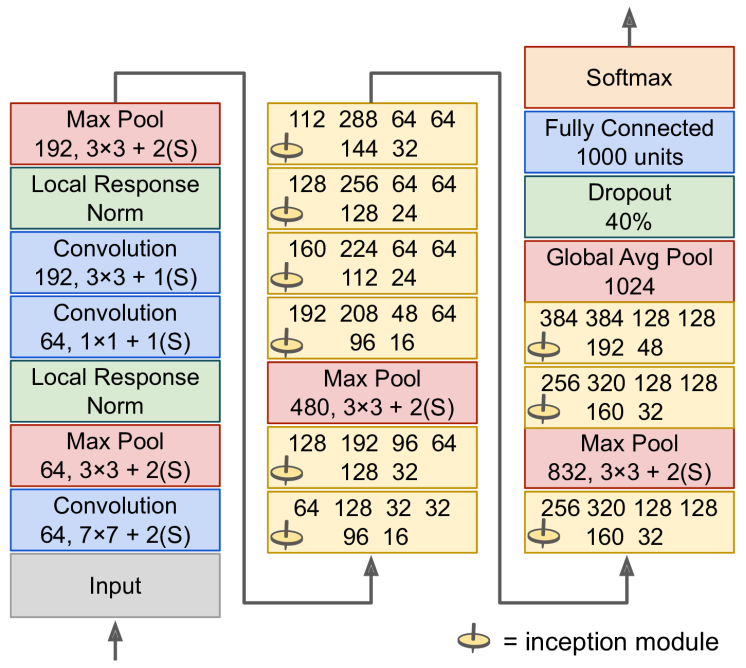
\includegraphics[width=.5\linewidth]{Images/GoogLeNet.png}
  \caption[Architecture of GoogLeNet]{Architecture of GoogLeNet. This massive CNN is GoogLeNet. The inception modules show the number of feature maps outputted by each of the convolutional layers in the inception modules. All convolutional layers use ReLU activation.}
  \label{fig:GoogLeNet}
\end{figure}
% subsubsection googlenet (end)

\subsubsection{VGGNet} % (fold)
\label{ssub:vggnet}
\begin{itemize}
  \item very simple classical architecture:
  \begin{itemize}
    \item 2 or 3 convolutional layers $\Longrightarrow$ pooling layer $\Longrightarrow$ 2 or 3 convolutional layers $\Longrightarrow$ pooling ... $\Longrightarrow$ dense layer with 2 hidden layers and output
    \item all filters were 3x3
  \end{itemize}
\end{itemize}
% subsubsection vggnet (end)

\subsubsection{ResNet} % (fold)
\label{ssub:resnet}
\begin{itemize}
  \item very deep model with 152 layers but few parameters
  \item the key is \textbf{residual learning}
  \begin{itemize}
    \item fig. \ref{fig:reslern} shows, the approach of residual learning:
    \newline \indent $\longrightarrow$ the input is added to the output of the model, resulting in the model having to learn $f(x) = h(x) - x$ rather than $f(x) = h(x)$, with $h(x)$ being the function we want to model
    \item as the weights are random in the beginning, the activation values will be close to 0, so $f(x) \approx 0$ in the early learning phases, thus $f(x) = h(x) - x \iff h(x) \approx x$, which is close to the input
    \newline \indent $\longrightarrow$ this allows to speed up the training process, because the learning process is a lot quicker in the beginning
    \item a network with many skip connections will be able to learn even if some of the convolutionaly layers have not started to learn yet
    \item a deep residual netweork can be seen as a stack of residual units, where each residual unit is a stamm neural network with a skip connection
    \item fig. \ref{fig:CNN_RNN} shows the primary advantage of using residual neural networks (i.e. empolying skip connections)
  \end{itemize}
  \item Fig. \ref{fig:ResNet} shows the architecture of the ResNet
  \item the structure is similar in that of the GoogLeNet when comparing the first and last layers. The main difference is the usage of residual units vs. inception units
  \item residual units are comprised of two convolutional layers (no pooling layer!) with Batch Noramlization and ReLU activation
  \newline \indent $\longrightarrow$ 3x3 kernels and preserving spatial dimensions
  \item number of feature maps is doubled every few residual units, when stride of 2 is used for one unit, halving width and height
  \newline \indent $\longrightarrow$ as this conflicts with the skip connection, which preserves its dimensions, the skip connection is passed through a convolutional layer with stride 2 and kernel size 1x1
  \item ResNet architectures are quite common, with ResNet-34 being a much employed model
  \newline \indent $\longrightarrow$ 34 layers (only counting convolutional and dense layers), with 3 residual units (RU) with 64 feat maps, 4 RUs with 128 maps, 6 RUs with 256 maps, and 3 RUs ith 512 maps
  \item larger ResNets than ResNet-34 tend to use RUs with 3 instead of 2 convolutional layers
\end{itemize}
\begin{figure}
  \centering
  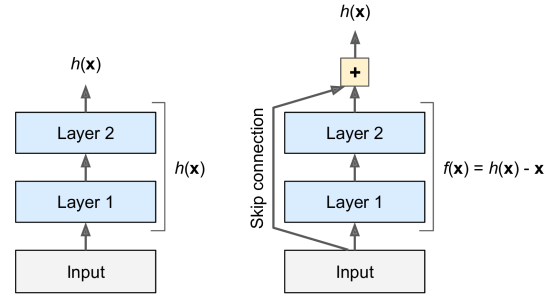
\includegraphics[width=.5\linewidth]{Images/residual_learning.png}
  \caption[Residual learning]{Residual learning. By skipping the modelled function a different function is learned which turns out to be advantageous.}
  \label{fig:reslern}
\end{figure}
\begin{figure}
  \centering
  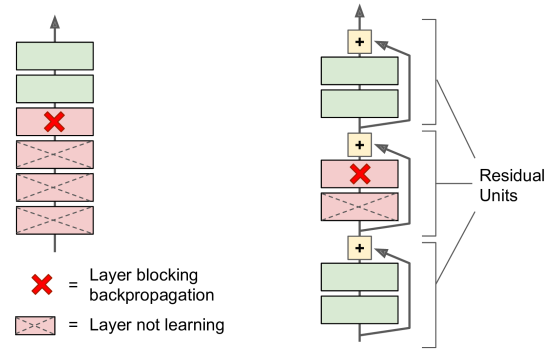
\includegraphics[width=.5\linewidth]{Images/CNN_RNN.png}
  \caption[Regular deep neural network vs. deep residual network]{Regular deep neural network vs. deep residual network. The left side shows a conventional deep neural network, where learning is not possible if one layer in the chain has not learned yet, blocking backpropagation, whereas the residual neural network can learn anyways, due to the skip connections.}
  \label{fig:CNN_RNN}
\end{figure}
\begin{figure}
  \centering
  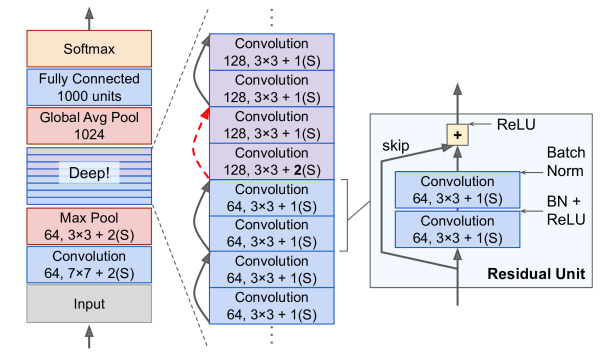
\includegraphics[width=.5\linewidth]{Images/ResNet.png}
  \caption[Architecture of ResNet]{Architecture of ResNet. Similar to GoogLeNet in the beginning and end, but with a lot of residual units in the middle in contrast to the inception units.}
  \label{fig:ResNet}
\end{figure}
% subsubsection resnet (end)

\subsubsection{Xception} % (fold)
\label{ssub:xception}
\begin{itemize}
  \item author of Keras (Francois Chollet) merged GoogLeNet and ResNet replacing inception modules with \textit{depthwise separable convolution} 
  \begin{itemize}
    \item fig. \ref{fig:seperable_convolution} shows a depthwise seperable convolutional layer, it takes an input (usually would not be used after the input, but rather further on in the network) and evaluates spatial-only filters (1 per input channel, further on in the network these correspond to feature maps) and at the same time applies depthwise-only filters finally connecting the two
    \item seperable convolutions use less parameters, les smemory, and less computations and usually perform better
  \end{itemize}
  \item the Xception network combines regular convolutional layers and the seperable convolution layers, thus combining methods of independently looking for cross-channel patterns as well as jointly. This has yielded strong results
\end{itemize}
\begin{figure}
  \centering
  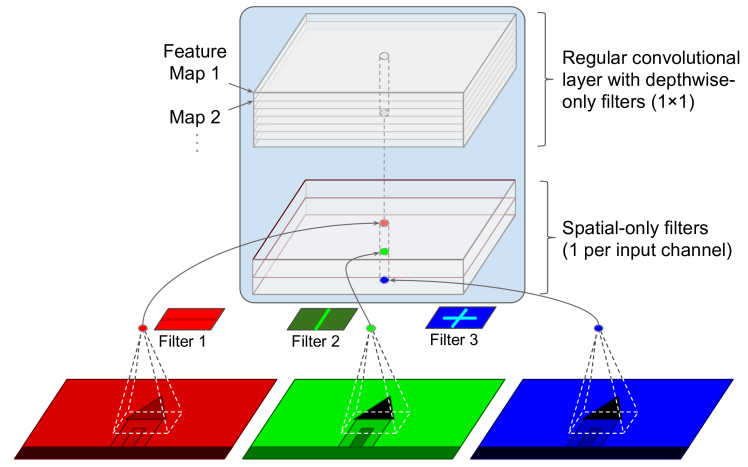
\includegraphics[width=.5\linewidth]{Images/seperable_convolution.png}
  \caption[Depthwise Seperable Convolution]{Depthwise Seperable Convolution is used to independently evalueate spatial and depthwise patterns contrary to regular convolutional layers that look at them jointly.}
  \label{fig:seperable_convolution}
\end{figure}
% subsubsection xception (end)

\subsubsection{SENet} % (fold)
\label{ssub:senet}
\begin{itemize}
  \item squeeze-and-Excitation Network - similar in structure to ResNets or inception networks, but the performance is boosted by the introduction of an \textbf{SE Block} to every unit in the original architecture
  \begin{itemize}
    \item fig. \ref{fig:seblock} shows in what way the SE Block is included in the original architecture
    \item a SE Block analyzes the output of the unit it's attached to
    \item only looks depth-wise
    \item sees what features are active together
    \item it applies the spatial concept of firing and wiring together and applies it to features
    \newline \indent $\longrightarrow$ if the features of eyes, noses and mouths always fire together and in one case only nose and mouth features fire up, the SE block will inhibit other irrelevant features to boost the eyes feature
    \newline \indent $\hookrightarrow$ this can be advantageous when there is something blocking an eye which can thereby be revealed
    \item fig. \ref{fig:seblock_recal} shows how the input feature map is multiplied by the recalibrated feature map, causing features that would otherwise pass unnoticed to be noticed
    \item SE Blocks are just composed of 3 elements:
    \newline \indent $\longrightarrow$ Global Average Pooling layer - gives out one value per feature map
    \newline \indent $\longrightarrow$ hidden dense layer using ReLU activation - vastly reduces dimension causing the SE Block to learn what belongs together (low dimensional vector representation -> embedding)
    \newline \indent $\longrightarrow$ dense output layer using sigmoid activation - takes embeddin and outputs recalibration vector with values between 0 and 1 per feature map
    \item irrelevant features get numbers close to 0 - get ignored, relevant features get values close to 1 - unity
  \end{itemize}
\end{itemize}
\begin{figure}
  \centering
  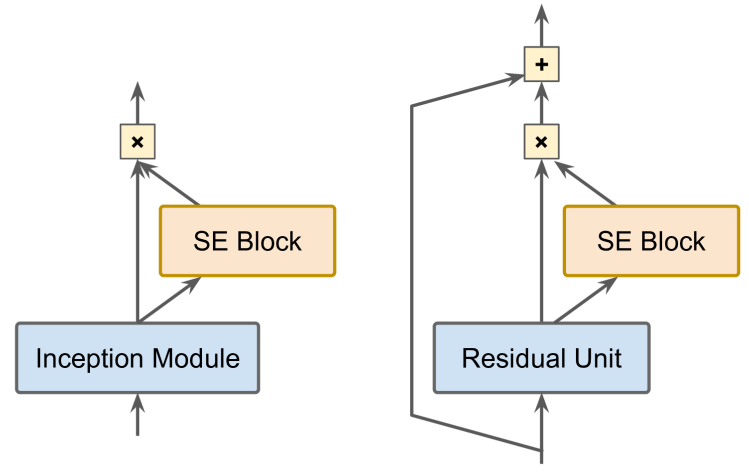
\includegraphics[width=.5\linewidth]{Images/SEBlock.png}
  \caption[SE-Block in inception modules and residual units]{SE-Block in inception modules and residual units. The introduction of this small neural network boosts the performance of the original network. }
  \label{fig:seblock}
\end{figure}
\begin{figure}
  \centering
  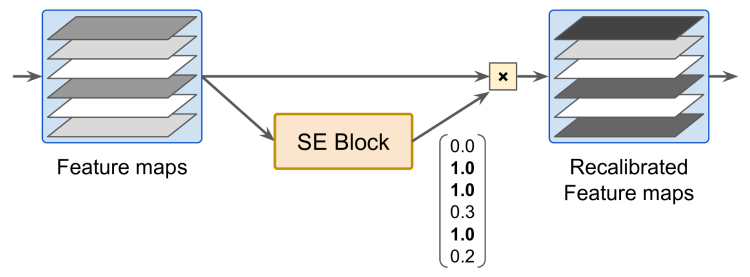
\includegraphics[width=.5\linewidth]{Images/seblock_recalibration.png}
  \caption[Recalibration by SE Block]{Recalibration by SE Block. This causes a boosting of features that would normally light up with other features, removing ambiguity.}
  \label{fig:seblock_recal}
\end{figure}
% subsubsection senet (end)


\subsubsection{Implementation of a ResNet-34 CNN Using Keras} % (fold)
\label{ssub:implementation_of_a_resnet_34_cnn_using_keras}
\begin{itemize}
  \item CNN implementation is straight forward for the shown models
  \item create standard convolutional layer first to not repeat every time:
  \begin{python}
    DefaultConv2D = partial(keras.layers.Conv2D, kernel_size = 3,
                            strides = 1, padding = 'SAME', use_bias = False)
  \end{python}
  \item create ResidualUnit layer
  \begin{python}
    class ResidualUnit(keras.layers.Layer):
      def __init__(self, filters, strides=1, 
                  activation="relu", **kwargs):
        super().__init__(**kwargs)
        self.activation = keras.activations.get(activation)

        self.main_layers = [
              DefaultConv2D(filters, strides=strides),
              keras.layers.BatchNormalization(),
              self.activation,
              DefaultConv2D(filters),
              keras.layers.BatchNormalization()
          ]
        
        self.skip_layers = []
        if strides > 1:
          self.skip_layers = [
            DefaultConv2D(filters, kernel_size=1, strides=strides),
                          keras.layers.BatchNormalization()
                          ]

      def call(self, inputs):
        Z = inputs
        for layer in self.main_layers:
          Z = layer(Z)

        skip_Z = inputs
        for layer in self.skip_layers:
          skip_Z = layer(skip_Z)

        return self.activation(Z + skip_Z)
  \end{python}
  \item now that the class is defined, every RU can be treated as a layer in a sequential model:
  \begin{python}
    model = keras.models.Sequential()
    model.add(DefaultConv2D(64, kernel_size=7, strides=2,
                            input_shape=[224, 224, 3]))

    model.add(keras.layers.BatchNormalization())
    model.add(keras.layers.Activation("relu"))
    model.add(keras.layers.MaxPool2D(pool_size=3, strides=2, padding="SAME"))

    prev_filters = 64
    for filters in [64] * 3 + [128] * 4 + [256] * 6 + [512] * 3:
        strides = 1 if filters == prev_filters else 2
        model.add(ResidualUnit(filters, strides=strides))
        prev_filters = filters

    model.add(keras.layers.GlobalAvgPool2D())
    model.add(keras.layers.Flatten())
    model.add(keras.layers.Dense(10, activation="softmax")) 
  \end{python}
  \item the iterable, that the for loop iterates through is necessary to get the correct number of feature maps for the RUs
  \item to make sure that the stride only gets increased on the third and last iteration of one feature map size, the if clause checks for filter == prev-filters
\end{itemize}
% subsubsection implementation_of_a_resnet_34_cnn_using_keras (end)
\subsubsection{Easy Guide to Predidctions with Pretrained Models} % (fold)
\label{ssub:easy_guide_to_predidctions_with_pretrained_models}

\begin{itemize}
  \item standard models like GoogLeNet or ResNet readily available through the keras API:
  \begin{python}
    model = keras.applications.resnet50.ResNet50(weights = 'imagenet')
  \end{python}
  \item this will yield a ResNet-50 model and download weights pretrained on the ImageNet dataset
  \newline \indent $\longrightarrow$ images have to have right size (224 x 224)
  \newline \indent $\longrightarrow$ resizing is possible with \begin{python}
    tf.image.resize(__your_images__, [__new_x_and_y_dimensions__])
    tf.image.crop_and_resize() # can be used in case preservation of aspect ratio is crucial
  \end{python}
  \item models have inherent preprocessing pipelines, to apply them to your inputs, your pixels in the images need a range from 0 - 255, 
  \newline \indent $\longrightarrow$ both can be achieved in one step:
  \begin{python}
    inputs = keras.applications.resnet50.preprocess_input(__your_images__ * 255) # assuming images where between 0 and 1
  \end{python}
  \item finally predictions can be made:
  \begin{python}
    Y_test = model.predict(inputs)
  \end{python}
  \item resulting Y-test is a matrix with dimensions = [number of images, number of classes]
  \item to decode the matrix and show the top k number of predictions:
  \begin{python}
    top_K = keras.applications.resnet50.decode_predictions(Y_proba, top=3)
    for image_index in range(len(images)):
        print("Image #{}".format(image_index))
        for class_id, name, y_proba in top_K[image_index]:
            print(" {} - {:12s} {:.2f}%".format(class_id, name, y_proba * 100))
        print()
  \end{python}
  \item this is a very easy setup to test pretrained models for your purpo(i)ses
\end{itemize}
% subsubsection easy_guide_to_predidctions_with_pretrained_models (end)

\subsubsection{Pretrained Models for Transfer Learning} % (fold)
\label{ssub:pretrained_models_for_transfer_learning}
\begin{itemize}
  \item when datasets of a pretrained model was too different from your dataset, but you still want to make use of their learning time, use \textbf{transfer learning}
  \item especially the lower levels can be resused, saving a lot of computational time
  \begin{python}
    import tensorflow_datasets as tfds

    dataset, info = tfds.load('tf_flowers', as_supervised = True
                              with_info = True)
    dataset_size  = info.splits["train"].num_examples # 3670
    class_names = info.features["label"].names # ["dandelion", 
                                                  "daisy", ...]
    n_classes = info.features["label"].num_classes # 5
  \end{python}
  \item this is a TensorFlow Dataset of flowers that we want to use in an Xception model to classify them
  \item we still need to split our dataset into train, test, and validation
  \begin{python}
    test, train, valid = tfds.Split.TRAIN.subsplit([10, 15, 75])

    test_set = tfds.load("tf_floswer", split = test, as_supervised = True)
    valid_set = tfds.load("tf_floswer", split = valid, as_supervised = True)
    train_set = tfds.load("tf_floswer", split = train, as_supervised = True) 
  \end{python}
  \item to make the images of the new dataset compatible with the model, the images  needs to be resized and the preprocess\_input function needs to be run:
  \begin{python}
    def preprocess(image, label):
        resized_image = tf.image.resize(image, [224, 224])
        final_image = keras.applications.xception.preprocess_input(resized_image)
        return final_image, label
  \end{python}
  \item now we apply the preprocessing to all 3 sets and shuffle train set, additionally we add batching and prefetching:
  \begin{python}
    batch_size = 32
    train_set = train_set.shuffle(1000).repeat()
    train_set = train_set.map(preprocess).batch(batch_size).prefetch(1)
    valid_set = valid_set.map(preprocess).batch(batch_size).prefetch(1)
    test_set = test_set.map(preprocess).batch(batch_size).prefetch(1)
  \end{python}
  \item at this stage optional augmentation methods could be introduced by replacing preprocess with other methods
  \newline \indent $\longrightarrow$ for example: tf.image.random\_crop() or tf.image.random\_flip\_left\_right()
  \item now that the input is ready, we load the Xception model without the global average pooling layer and the dense output layer, instead we add our own
  \begin{python}
    base_model = keras.applications.xception.Xception(weights="imagenet",
                                                      include_top=False)
    avg = keras.layers.GlobalAveragePooling2D()(base_model.output)
    output = keras.layers.Dense(n_classes, activation="softmax")(avg)
    model = keras.models.Model(inputs=base_model.input, outputs=output)

    for layer in base_model.layers:
        layer.trainable = False
  \end{python}
  \item the last part is important to freeze the weights while we train our new layers, this will be changed after a while
  \item finally the training is performed:
  \begin{python}
    optimizer = keras.optimizers.SGD(lr=0.2, momentum=0.9, decay=0.01)
    model.compile(loss="sparse_categorical_crossentropy", 
                  optimizer=optimizer, metrics=["accuracy"])
    history = model.fit(train_set,
                steps_per_epoch=int(0.75 * dataset_size / batch_size),
                validation_data=valid_set,
                validation_steps=int(0.15 * dataset_size / batch_size),
                epochs=5)
  \end{python}
  \item after a while the validation accuracy should reach 75-80\%, and stagnate, indicating that the top layers are well trained and it's time to unfreeze the weights:
  \begin{python}
    for layer in base_model.layers:
        layer.trainable = True

    optimizer = keras.optimizers.SGD(lr=0.01, momentum=0.9, decay=0.001)
    model.compile(...)
    history = model.fit(...)
  \end{python}
  \item the recompiling of the model is necessary for the changes to take effect
  \item the learning rate is far lower than before to make sure that the top layer weights don't get ruined again
  \item using all hidden layers except for the output layer of a pretrained model
  \begin{python}
    model_A = keras.models.load_model("my_model_A.h5")
    model_B_on_A = keras.models.Sequential(model_A.layers[:-1])
    model_B_on_A.add(keras.layers.Dense(1, activation="sigmoid"))
    # the above method will also alter model_A when training, 
    # if that is a problem, do the following:
    model_A_clone = keras.models.clone_model(model_A)
    model_A_clone.set_weights(model_A.get_weights())
  \end{python}
  \item the output layer of model\_B\_on\_A needs to be trained while the other layers need to remain the same:
  \begin{python}
    for layer in model_B_on_A.layers[:-1]:
        layer.trainable = False
    model_B_on_A.compile(loss="binary_crossentropy", 
                          optimizer="sgd",
                          metrics=["accuracy"])
  \end{python}
\end{itemize}
% subsubsection pretrained_models_for_transfer_learning (end)

% subsubsection convolutional_neural_networks_ (end)

% subsubsection basic_structure (end)






%____________________________________________Ende dieser Sitzung__________________________________________________


%_______________________________________Thema und Datum dieser Sitzung____________________________________________
\newpage
\section{Taxonomy}
\addtocounter{section}{1}
Datum: 04.Mai \ 

\noindent\hrulefill  \

%__________________________________________Inhalt dieser Sitzung__________________________________________________

\subsection{Pfad zu Kateceanen} % (fold)
\label{sub:Pfad zu Kateceanen}

\begin{itemize}
  \item hierarchy of taxonomic ranks: 
  \newline \indent $\longrightarrow$ Life $\Longrightarrow$ Domain $\Longrightarrow$ Kingdom $\Longrightarrow$ Phylum $\Longrightarrow$ Class $\Longrightarrow$ Order $\Longrightarrow$ Family $\Longrightarrow$ Genus $\Longrightarrow$ Species
  \item Rangstufen der Taxonomie: 
  \newline \indent $\longrightarrow$ Lebewesen $\Longrightarrow$ Domäne $\Longrightarrow$ Reich $\Longrightarrow$ Stamm $\Longrightarrow$ Klasse $\Longrightarrow$ Ordnung $\Longrightarrow$ Familie $\Longrightarrow$ Gattung $\Longrightarrow$ Art
 \item Animalia (Kingdom) $\Longrightarrow$ Chordata (Phylum) $\Longrightarrow$ Mammalia (Class) $\Longrightarrow$ Artiodactyla (also even-toed ungulates $\Longrightarrow$ lollinger) (Order)
 \item Tierreich (Reich) $\Longrightarrow$ Chordatiere (Stamm) $\Longrightarrow$ Säugetiere (Klasse) $\Longrightarrow$ Laurasiatheria (Überordnung)
   \item Catecean (Infraorder)
   \item Katecean (Ordnung) 
   \newline \indent $\hookrightarrow$ (umgangssprachl. Wal, wobei Wale eignetlich nur bartenwale bezeihnen)
\end{itemize}


\subsection{Cetaceans} % (fold)
\label{sub:cetaceans}

\subsubsection{Baleen whale (mysticetes) (Parvorder) - Bartenwale (Unterordnung)} % (fold)
\label{ssub:baleen_whale_mysticetes_parvorder_bartenwale_unterordnung_}

% subsubsection baleen_whale_mysticetes_parvorder_bartenwale_unterordnung_ (end)
\textbf{Rorqual (balaenopteridae) (Family) - Furchenwale (Familie)}
\begin{itemize}
  \item Megaptera (Genus) - Megaptera (Gattung) 
  \newline \indent $\hookrightarrow$ verfügt nur über eine Art, den Buckelwal
      \newline \indent $\longrightarrow$ Humpback whale (Species) - Buckelwal (Art)
\end{itemize}
\begin{itemize}
  \item Balaenoptera (Genus) - Balaenoptera (Gattung)
    \newline \indent $\longrightarrow$ Blue whale (Species) - Blauwal (Art)
    \newline \indent $\longrightarrow$ Minke whale (Species) - Zwergwal (Art)
    \newline \indent $\longrightarrow$ Fin whale (Species) - Finnwal (Art)
    \newline \indent $\hookrightarrow$ second longest animal after blue whale 
\end{itemize}

\textbf{Balaenidae (Family) - Glattwale (Familie) }
\newline \indent $\hookrightarrow$ wurden am stärksten durch Jagen dezimiert
\begin{itemize}
  \item Right whale (eubalaena) (Genus) - Eubalaena (Gattung)
    \newline \indent $\longrightarrow$ North atlantic right whale (eubalaena glacialis) (Species) - Atlantischer Nordkaper (Art)

  \item Balaena (Genus)
    \newline \indent $\longrightarrow$ Bowhead whale (balaena mysticetus) (Species) - Grönlandwal (Art)
\end{itemize}

\subsubsection{Toothed whale (odontocetes) (Parvorder) - Zahnwale (Unterordnung)} % (fold)
\label{ssub:toothed_whale_odontocetes_parvorder_zahnwale_unterordnung_}
\indent $\longrightarrow$ (- Delphinida (Clade) )
\newline \indent $\longrightarrow$ (- Delphinoidae (Superfamily) - Delfinartige (Überfamilie)) \\
\textbf{Oceanic dolphins (delphinidae) (Family) - Delfine (Familie)}
\begin{itemize}
  \item Orcinus (Genus) - Orcinus (Gattung)
    \newline \indent $\longrightarrow$ Orca or killer whale (Species) - Schwertwal auch Orca, Killerwal (Art)
\end{itemize}

\indent $\longrightarrow$ (- Physeteroidea (Superfamily)) \\
\textbf{Physeteridae (Family)}
\begin{itemize}
  \item Physeter (Genus)
    \newline \indent $\longrightarrow$ Sperm whale (physeter macrocephalus) (Species) - Pottwal (Art)
    \newline \indent $\hookrightarrow$ largest toothed animal 
\end{itemize}
% subsubsection toothed_whale_odontocetes_parvorder_zahnwale_unterordnung_ (end)

% subsubsection cetaceans (end)

%____________________________________________Ende dieser Sitzung__________________________________________________



% ar snippet für \longrightarrow
% iar snippet für \indent   \
% hkar snippet für \hookrightarrow
% ihkar snippet für \indent \hookrightarrow \{}

\bibliography{/mnt/swap/Studium/Master/Masterarbeit/Protokoll/lit_af/MastersThesisBib}
% \bibliography{lit_af/MastersThesisBib}
\noindent\hrulefill
\end{document}